\documentclass[]{article}
\usepackage{lmodern}
\usepackage{amssymb,amsmath}
\usepackage{ifxetex,ifluatex}
\usepackage{fixltx2e} % provides \textsubscript
\ifnum 0\ifxetex 1\fi\ifluatex 1\fi=0 % if pdftex
  \usepackage[T1]{fontenc}
  \usepackage[utf8]{inputenc}
\else % if luatex or xelatex
  \ifxetex
    \usepackage{mathspec}
  \else
    \usepackage{fontspec}
  \fi
  \defaultfontfeatures{Ligatures=TeX,Scale=MatchLowercase}
\fi
% use upquote if available, for straight quotes in verbatim environments
\IfFileExists{upquote.sty}{\usepackage{upquote}}{}
% use microtype if available
\IfFileExists{microtype.sty}{%
\usepackage{microtype}
\UseMicrotypeSet[protrusion]{basicmath} % disable protrusion for tt fonts
}{}
\usepackage[margin=1in]{geometry}
\usepackage{hyperref}
\hypersetup{unicode=true,
            pdftitle={Tarea 3},
            pdfborder={0 0 0},
            breaklinks=true}
\urlstyle{same}  % don't use monospace font for urls
\usepackage{color}
\usepackage{fancyvrb}
\newcommand{\VerbBar}{|}
\newcommand{\VERB}{\Verb[commandchars=\\\{\}]}
\DefineVerbatimEnvironment{Highlighting}{Verbatim}{commandchars=\\\{\}}
% Add ',fontsize=\small' for more characters per line
\usepackage{framed}
\definecolor{shadecolor}{RGB}{248,248,248}
\newenvironment{Shaded}{\begin{snugshade}}{\end{snugshade}}
\newcommand{\AlertTok}[1]{\textcolor[rgb]{0.94,0.16,0.16}{#1}}
\newcommand{\AnnotationTok}[1]{\textcolor[rgb]{0.56,0.35,0.01}{\textbf{\textit{#1}}}}
\newcommand{\AttributeTok}[1]{\textcolor[rgb]{0.77,0.63,0.00}{#1}}
\newcommand{\BaseNTok}[1]{\textcolor[rgb]{0.00,0.00,0.81}{#1}}
\newcommand{\BuiltInTok}[1]{#1}
\newcommand{\CharTok}[1]{\textcolor[rgb]{0.31,0.60,0.02}{#1}}
\newcommand{\CommentTok}[1]{\textcolor[rgb]{0.56,0.35,0.01}{\textit{#1}}}
\newcommand{\CommentVarTok}[1]{\textcolor[rgb]{0.56,0.35,0.01}{\textbf{\textit{#1}}}}
\newcommand{\ConstantTok}[1]{\textcolor[rgb]{0.00,0.00,0.00}{#1}}
\newcommand{\ControlFlowTok}[1]{\textcolor[rgb]{0.13,0.29,0.53}{\textbf{#1}}}
\newcommand{\DataTypeTok}[1]{\textcolor[rgb]{0.13,0.29,0.53}{#1}}
\newcommand{\DecValTok}[1]{\textcolor[rgb]{0.00,0.00,0.81}{#1}}
\newcommand{\DocumentationTok}[1]{\textcolor[rgb]{0.56,0.35,0.01}{\textbf{\textit{#1}}}}
\newcommand{\ErrorTok}[1]{\textcolor[rgb]{0.64,0.00,0.00}{\textbf{#1}}}
\newcommand{\ExtensionTok}[1]{#1}
\newcommand{\FloatTok}[1]{\textcolor[rgb]{0.00,0.00,0.81}{#1}}
\newcommand{\FunctionTok}[1]{\textcolor[rgb]{0.00,0.00,0.00}{#1}}
\newcommand{\ImportTok}[1]{#1}
\newcommand{\InformationTok}[1]{\textcolor[rgb]{0.56,0.35,0.01}{\textbf{\textit{#1}}}}
\newcommand{\KeywordTok}[1]{\textcolor[rgb]{0.13,0.29,0.53}{\textbf{#1}}}
\newcommand{\NormalTok}[1]{#1}
\newcommand{\OperatorTok}[1]{\textcolor[rgb]{0.81,0.36,0.00}{\textbf{#1}}}
\newcommand{\OtherTok}[1]{\textcolor[rgb]{0.56,0.35,0.01}{#1}}
\newcommand{\PreprocessorTok}[1]{\textcolor[rgb]{0.56,0.35,0.01}{\textit{#1}}}
\newcommand{\RegionMarkerTok}[1]{#1}
\newcommand{\SpecialCharTok}[1]{\textcolor[rgb]{0.00,0.00,0.00}{#1}}
\newcommand{\SpecialStringTok}[1]{\textcolor[rgb]{0.31,0.60,0.02}{#1}}
\newcommand{\StringTok}[1]{\textcolor[rgb]{0.31,0.60,0.02}{#1}}
\newcommand{\VariableTok}[1]{\textcolor[rgb]{0.00,0.00,0.00}{#1}}
\newcommand{\VerbatimStringTok}[1]{\textcolor[rgb]{0.31,0.60,0.02}{#1}}
\newcommand{\WarningTok}[1]{\textcolor[rgb]{0.56,0.35,0.01}{\textbf{\textit{#1}}}}
\usepackage{longtable,booktabs}
\usepackage{graphicx,grffile}
\makeatletter
\def\maxwidth{\ifdim\Gin@nat@width>\linewidth\linewidth\else\Gin@nat@width\fi}
\def\maxheight{\ifdim\Gin@nat@height>\textheight\textheight\else\Gin@nat@height\fi}
\makeatother
% Scale images if necessary, so that they will not overflow the page
% margins by default, and it is still possible to overwrite the defaults
% using explicit options in \includegraphics[width, height, ...]{}
\setkeys{Gin}{width=\maxwidth,height=\maxheight,keepaspectratio}
\IfFileExists{parskip.sty}{%
\usepackage{parskip}
}{% else
\setlength{\parindent}{0pt}
\setlength{\parskip}{6pt plus 2pt minus 1pt}
}
\setlength{\emergencystretch}{3em}  % prevent overfull lines
\providecommand{\tightlist}{%
  \setlength{\itemsep}{0pt}\setlength{\parskip}{0pt}}
\setcounter{secnumdepth}{0}
% Redefines (sub)paragraphs to behave more like sections
\ifx\paragraph\undefined\else
\let\oldparagraph\paragraph
\renewcommand{\paragraph}[1]{\oldparagraph{#1}\mbox{}}
\fi
\ifx\subparagraph\undefined\else
\let\oldsubparagraph\subparagraph
\renewcommand{\subparagraph}[1]{\oldsubparagraph{#1}\mbox{}}
\fi

%%% Use protect on footnotes to avoid problems with footnotes in titles
\let\rmarkdownfootnote\footnote%
\def\footnote{\protect\rmarkdownfootnote}

%%% Change title format to be more compact
\usepackage{titling}

% Create subtitle command for use in maketitle
\providecommand{\subtitle}[1]{
  \posttitle{
    \begin{center}\large#1\end{center}
    }
}

\setlength{\droptitle}{-2em}

  \title{Tarea 3}
    \pretitle{\vspace{\droptitle}\centering\huge}
  \posttitle{\par}
    \author{}
    \preauthor{}\postauthor{}
    \date{}
    \predate{}\postdate{}
  

\begin{document}
\maketitle


\includegraphics{banner.png}

Tarea 3: Frequentist Inference II

CC6104: Statistical Thinking

\hypertarget{integrantes}{%
\paragraph{\texorpdfstring{\textbf{Integrantes
:}}{Integrantes :}}\label{integrantes}}

\begin{itemize}
\tightlist
\item
  Rafael De La Sotta
\item
  Felipe Ortúzar
\end{itemize}

\hypertarget{cuerpo-docente}{%
\paragraph{\texorpdfstring{\textbf{Cuerpo
Docente:}}{Cuerpo Docente:}}\label{cuerpo-docente}}

\begin{itemize}
\tightlist
\item
  Profesor: Felipe Bravo M.
\item
  Auxiliar: Sebastian Bustos e Ignacio Meza D.
\end{itemize}

\hypertarget{fecha-limite-de-entrega}{%
\paragraph{\texorpdfstring{\textbf{Fecha límite de
entrega:}}{Fecha límite de entrega:}}\label{fecha-limite-de-entrega}}

\hypertarget{indice}{%
\subsubsection{\texorpdfstring{\textbf{Índice:}}{Índice:}}\label{indice}}

\begin{enumerate}
\def\labelenumi{\arabic{enumi}.}
\tightlist
\item
  \protect\hyperlink{id1}{Objetivo}
\item
  \protect\hyperlink{id2}{Instrucciones}
\item
  \protect\hyperlink{id3}{Referencias}
\item
  \protect\hyperlink{id4}{Primera Parte: Preguntas Teóricas}
\item
  \protect\hyperlink{id5}{Segunda Parte: Elaboración de Código}
\end{enumerate}

\hypertarget{objetivo}{%
\subsubsection{\texorpdfstring{\textbf{Objetivo}}{Objetivo}}\label{objetivo}}

\href{mailto:Bienvenid@s}{\nolinkurl{Bienvenid@s}} a la tercera tarea
del curso Statistical Thinking. Esta tarea tiene como objetivo evaluar
los contenidos teóricos de la segunda parte del curso, los cuales se
enfocan principalmente en el diseño de experimentos, test de hipótesis y
regresión lineal. Si aún no han visto las clases, se recomienda visitar
los enlaces de las referencias.

La tarea consta de una parte teórica que busca evaluar conceptos vistos
en clases. Seguido por una parte práctica con el fin de introducirlos a
la programación en R enfocada en el análisis estadístico de datos.

\hypertarget{instrucciones}{%
\subsubsection{\texorpdfstring{\textbf{Instrucciones:}}{Instrucciones:}}\label{instrucciones}}

\begin{itemize}
\tightlist
\item
  La tarea se realiza en grupos de \textbf{máximo 2 personas}. Pero no
  existe problema si usted desea hacer de forma individual.
\item
  La entrega es a través de u-cursos a más tardar el día estipulado en
  la misma plataforma. A las tareas atrasadas se les descontará un punto
  por día.
\item
  El formato de entrega es este mismo \textbf{Rmarkdown} y un
  \textbf{html} con la tarea desarrollada. Por favor compruebe que todas
  las celdas han sido ejecutadas en el archivo html.
\item
  Al momento de la revisión tu código será ejecutado. Por favor verifica
  que tu entrega no tenga errores de compilación.
\item
  No serán revisadas tareas desarrolladas en Python.
\item
  Está \textbf{PROHIBIDO} la copia o compartir las respuestas entre
  integrantes de diferentes grupos.
\item
  Pueden realizar consultas de la tarea a través de U-cursos y/o del
  canal de Discord del curso.
\end{itemize}

\hypertarget{referencias}{%
\subsubsection{\texorpdfstring{\textbf{Referencias:}}{Referencias:}}\label{referencias}}

Slides de las clases:

\begin{itemize}
\tightlist
\item
  \href{https://github.com/dccuchile/CC6104/blob/master/slides/ST-hypothesis.pdf}{Design
  of Experiments \& Hypothesis Testing}
\item
  \href{https://github.com/dccuchile/CC6104/blob/master/slides/ST-regression.pdf}{Linear
  Regression}
\end{itemize}

Enlaces a videos de las clases:

\begin{itemize}
\tightlist
\item
  Design of Experiments \& Hypothesis Testing:
  \href{https://youtu.be/3MueyHnNNig}{video1}
  \href{https://youtu.be/JuyIrya23E0}{video2}
  \href{https://youtu.be/OXTyG6DIvK4}{video3}
  \href{https://youtu.be/95QeSwrNoLI}{video4}
  \href{https://youtu.be/ZCr3WCdc-54}{video5}
  \href{https://youtu.be/T6ZR0KoKhBQ}{video6}
\item
  Introduction to Statistical Inference:
  \href{https://youtu.be/ZLZXJPKH6tU}{video1}
  \href{https://youtu.be/mW7bHkJBcB4}{video2}
  \href{https://youtu.be/SHa5Neb7bfg}{video3}
  \href{https://youtu.be/rCD_jofxecY}{video4}
  \href{https://youtu.be/ir4P_f3s44g}{video5}
  \href{https://youtu.be/wfNhJWHPOi8}{video6}
\end{itemize}

\hypertarget{primera-parte-preguntas-teoricas}{%
\section{Primera Parte: Preguntas
Teóricas}\label{primera-parte-preguntas-teoricas}}

A continuación, se presentaran diferentes preguntas que abordan las
temáticas vistas en clases. Por favor responda cada una de estas de
forma breve.

\hypertarget{pregunta-1}{%
\paragraph{\texorpdfstring{\textbf{Pregunta
1:}}{Pregunta 1:}}\label{pregunta-1}}

Determine si las siguientes regresiones son lineales para los parámetros
\(\beta_{i}\)

\begin{itemize}
\item[$\square$]
  \(y(x) = \beta_{0} + \beta_{1} x\)
\item[$\square$]
  \(y(x) = \beta_{0} + \beta_{1} x + (\beta_{3}+x)^{3}\)
\item[$\square$]
  \(y(x) = \ln(x^{2}+\beta_{0})\)
\end{itemize}

\begin{quote}
Para que una expresión multivariable sea lineal se debe asegurar que
pueda ser expresada de forma matricial, \(Y = X \beta\).
\end{quote}

\begin{quote}
En el primer caso, \(y(x) = \beta_{0} + \beta_{1} x\) puede ser
expresada como:
\[ Y(x) =  \left( \begin{array}{ll} \beta_{0} \\ \beta_{1} \end{array} \right)^T \left( \begin{array}{ll} 1 \\ x \end{array} \right) \]
\end{quote}

\begin{quote}
Para el caso dos, este tiene a \(\beta^2\) y \(\beta^3\), como
consecuencia del cubo del binomio. Con esto valores es imposible
expresar la función como \(Y = X \beta\).
\end{quote}

\begin{quote}
Para el caso tres, este tiene una función logarítnica que impide separar
a \(\beta_{0}\) del resto de las expresiones y tambien impide expresar a
la función como \(Y = X \beta\).
\end{quote}

\hypertarget{pregunta-2}{%
\paragraph{\texorpdfstring{\textbf{Pregunta
2:}}{Pregunta 2:}}\label{pregunta-2}}

Una universidad esta interesada en saber cuantos alumnos gustan del
anime, para esto realiza una recopilación de datos y llega a la
construcción del siguiente modelo lineal simple:

\[\hat{N°\_de\_fanaticos\_del\_anime}=300+90*numero\_de\_semestres\]

¿Como podemos interpretar el intercepto y pendiente del modelo?, ¿El
intercepto y la pendiente tienen una interpretación coherente para
cualquier modelo lineal?, si no es así, de un ejemplo.

\begin{quote}
El intercepto sería la cantidad de estudiantes, fánaticos del anime, que
todavían no han cursado algún semestre en la universidad (0 semestres;
proto-mechones coloquialmente). Y la pendiente sería cuánto aumenta la
cantidad de estudiantes fanáticos del anime por cada semestre cursado en
la universidad. En modelos de la vida real hay que tener cierto cuidado
en los límites del modelo lineal, esto es, cuando el dominio o el
recorrido valen 0. Por ejemplo, si una panadería tiene este modelo
lineal para sus ventas: \#Ventas = 100 + 10 * \#Panes cocinados,
entonces, eso significa que cuando no cocinan panes tienen 100 ventas?
No, y es en casos como estos en donde se pierde la interpretación del
modelo lineal.
\end{quote}

\hypertarget{pregunta-3}{%
\paragraph{\texorpdfstring{\textbf{Pregunta
3:}}{Pregunta 3:}}\label{pregunta-3}}

Considere un test con dos muestras no aparejado, explique porque se hace
una corrección a los grados de libertad en el test de Welsh.

\begin{quote}
El test de Welsh se utiliza para, al asignar grados de libertad,
``castigar'' diferencias entre números de conjuntos de test de dos
muestras. Si se utilisa el métono común (n-m) no influiye que cantidad
de datos tiene cada conjunto, siendo esto de extrema relevancia para
casos desiguales.
\end{quote}

\begin{quote}
Por ejemplo, si se tiene un test de dos muestras donde una muestra tiene
muchos datos y la otra muy pocos. Para el método común, se tendría una
gran confianza en los datos dado la cantidad total de los datos, lo
cual, como sabemos, no sería correcto.
\end{quote}

\hypertarget{pregunta-4}{%
\paragraph{\texorpdfstring{\textbf{Pregunta
4:}}{Pregunta 4:}}\label{pregunta-4}}

Al realizar una regresión lineal simple con una variable categórica
\((\beta_{0} + \beta_{1} \cdot \text{categroica})\) ¿que interpretación
puede obtenerse del coeficiente que acompaña a la variable categórica?

\begin{quote}
La interpretación de la variable \(\beta_{1}\) es que corresponde a la
diferencia entre valores de cada grupo en esa categoría. Por ejemplo, en
un dataset con una categoría de ``deportistas'' y ``no deportistas'',
una columna ``proteína diaria ingerida'' y otra ``masa muscular'', y
considerando la función lineal:
\(Masa \, muscular = \beta_{0} + \beta_{1} \cdot proteína \, diaria \, ingerida\),
entonces \(\beta_{1}\) sería igual a la diferencia entre la proteína
diaria ingerida de los deportistas y los no deportistas. Cabe destacar
que la interpretación de \(\beta_{1}\) en el modelo implica que se está
realizando un test de hipótesis sobre las variables que definen a la
variable objetivo.
\end{quote}

\hypertarget{pregunta-5}{%
\paragraph{\texorpdfstring{\textbf{Pregunta
5:}}{Pregunta 5:}}\label{pregunta-5}}

Discuta la siguiente frase:

" Hacer una regresión lineal mediante máxima verosimilitud requiere
tener ciertas hipótesis probabilisticas de los datos, mientras que una
regresión realizada mediante mínimos cuadrados no necesita tener ninguna
hipótesis probabilista. "

\begin{quote}
Es importante saber que ambos métodos son equivalentes. En una regresión
lineal la máxima verosimilitud se alcanza solo si se minimiza el error
cuadratico medio, y vice versa. De hecho, por medio del método de máxima
veosilitud se obtiene que se debe minimizar el error cuadrático en una
regresión, y para esto se asume la distribución del error de esta. Y
para utilizar este método se realizan asumen los siguientes puntos:
\end{quote}

\begin{itemize}
\tightlist
\item
  Linealidad de los datos
\item
  error con distribución gausiana
\item
  varianza del error constante
\item
  Error independiente
\end{itemize}

\begin{quote}
Como consecuencia de todo lo anterior, podemos decir que al utilizar la
minimización del error cuadrado se están haciendo las mismas hipótesis
realizadas para linealizar mediante máxima verosimilitud.
\end{quote}

\hypertarget{pregunta-6}{%
\paragraph{\texorpdfstring{\textbf{Pregunta
6:}}{Pregunta 6:}}\label{pregunta-6}}

Explique porque el test de significancia sobre los parámetros de una
regresión lineal se realiza bajo la hipótesis nula \(\beta_{H_{0}}=0\).

\begin{quote}
Principalmente porque se desea \emph{rechazar} la hipótesis nula de que
\(\beta_{H_{0}}=0\) para \(\beta_0\) o ``intercepto'' y \(\beta_1\) o
``la pendiente''. Entonces, al rechazar la hipótesis nula de que
\(\beta_0 = 0\) se está ``diciendo'' que al inicio de la función, en
\(x=0\), el valor es muy diferente de 0 con cierto nivel de confianza.
Por otro lado, al rechazar la hipótesis nula de que \(\beta_1 = 0\),
significa que existe una relación lineal entre la variable y el
objetivo.
\end{quote}

\hypertarget{pregunta-7}{%
\paragraph{\texorpdfstring{\textbf{Pregunta
7:}}{Pregunta 7:}}\label{pregunta-7}}

¿Que nos dice la equivalencia de la máxima verosimilitud sobre los
parámetros que componen una regresión lineal? ¿Qué nos permitirían
calcular?

\begin{quote}
Asumiendo que el error entre la regresión lineal y los valores reales
tiene un distribución gaussiana, se busca la máxima verosimilitud para
este, la cual se alcanza cuando la suma de los errores cuadraticos es
mínima.
\end{quote}

\begin{quote}
Luego, los parámetros de linealización son escogidos de acuerdo a
minimizar el error cuadrático medio.
\end{quote}

\begin{quote}
Por ejemplo, para una regresión simple, se quiere tiene la siguiente
linealización:
\end{quote}

\[
h(x) = \beta_{0} + \beta_{1} \cdot x
\]

\begin{quote}
Los parámetros escogidos deben ser los que minimicen el error cuadratico
entre los datos reales y, y h(x).
\end{quote}

\[
SSE = \sum_{i}^{n}(y - h(x))
\]

\begin{quote}
En este caso, los parámetros que minimizan este errro son los
siguientes:
\end{quote}

\[
\hat{\beta_{1}} = \frac{\sum_{i}^{n}(x_i - \bar{x}) (y_i - \bar{y})}{\sum_{i}^{n}(x_i - \bar{x})^2}
\]

\[
\hat{\beta_{0}} = \bar{y} - \hat{\beta_{1}} \cdot \bar{x}
\]

\hypertarget{pregunta-8}{%
\subsubsection{\texorpdfstring{\textbf{Pregunta
8}}{Pregunta 8}}\label{pregunta-8}}

Consideremos una regresión lineal de una variable. En vez de mínimos
cuadrados es posible minimizar la expresión

\[
\displaystyle{\sum_{i=1}^{n}}|y_{i}-\beta_{0}-\beta_{1}x_{i}|
\] Explique en que se diferencia con mínimos cuadrados, de una posible
ventaja y desventaja de este método (en comparación a mínimos
cuadrados).

\begin{quote}
En primer lugar, hay que analizar qué ocurre cuando intentamos resolver
analíticamente la solución de encontrar el mínimo error. Lamentablemente
no existe una solución analítica debido a la presencia de la función
absoluto sobre los betas. En particular, \(\beta_0\) no tiene solución
(\(-n = 0\) o\(n = 0\)) y hay que cambiar la aproximación de la solución
a una de carácter iterativo. Estos dos problemas, (1) sin solución
analítica y (2) cálculo de la solución de manera iterativa, se
consideran desventajas. Además es posible que existan múltiples
soluciones, dependiendo de los datos.
\end{quote}

\begin{quote}
Por otro lado, el uso de valor absoluto para el cálculo del error
constituye una ventaja, al presentar mayor robustez frente a
\(\textit{outliers}\), ya que valores extremadamente grandes en
comparación a la media ya no van a generar desviaciones aún mayores (al
quedar al cuadrado).
\end{quote}

\hypertarget{pregunta-9}{%
\paragraph{\texorpdfstring{\textbf{Pregunta
9:}}{Pregunta 9:}}\label{pregunta-9}}

Explique porque el coeficiente \(R^2\) tiende a crecer con el numero de
variables.

\begin{quote}
Existen muchas maneras de expresar este termino, una de ellas es
\(R^{2} = 1 - \frac{SSE}{SST}\). Tal como sabemos, el término a
minimizar corresponde a SSE, por lo que este, si bien aumenta
constantemente, al ser la variable minimizada debiese aumentar a una
tasa menor que SST, el cual no es controlado por la regresión y tambien
aumenta constantemente.
\end{quote}

\begin{quote}
Dicho esto, se entiende que \(\frac{SSE}{SST}\) tiende a decrecer, y
producto de esto R tiende a aumentar su valor.
\end{quote}

\hypertarget{pregunta-10}{%
\paragraph{\texorpdfstring{\textbf{Pregunta
10}}{Pregunta 10}}\label{pregunta-10}}

Un estudio de cáncer realizado por la institución X ha señalado que las
personas que beben café poseen mayores probabilidades de padecer algún
cáncer pulmonar. El estudio causo un gran revuelo en la población, por
lo que una segunda institución ha decidido replicar el experimento,
llegando a la conclusión que las personas que toman café tienden a fumar
cigarrillos mientras beben esta bebida. Señale que tipo de variable
serían los fumadores de cigarrillos en el estudio de cáncer pulmonar y
explique cual es la característica de estas variables.

\begin{quote}
En este caso los fumadores de cigarrillos corresponde a una
\emph{variable de confusión}. Las variables de confusión son factores
que no son claros al iniciar un experimento, pero al ser identificadas
explican la relación entre otras dos o más variables que
``inexplicablemente'' estaban relacionadas, y esta variable de confusión
es aquella que explica la conexión.
\end{quote}

\begin{center}\rule{0.5\linewidth}{0.5pt}\end{center}

\hypertarget{segunda-parte-elaboracion-de-codigo}{%
\section{Segunda Parte: Elaboración de
Código}\label{segunda-parte-elaboracion-de-codigo}}

En la siguiente sección deberá resolver cada uno de los experimentos
computacionales a través de la programación en R. Para esto se le
aconseja que cree funciones en R, ya que le facilitará la ejecución de
gran parte de lo solicitado.

Para el desarrollo preste mucha atención en los enunciados, ya que se le
solicitará la implementación de métodos sin uso de funciones
predefinidas. Por otro lado, Las librerías permitidas para desarrollar
de la tarea 3 son las siguientes:

\begin{Shaded}
\begin{Highlighting}[]
\CommentTok{\# Manipulación de estructuras}
\FunctionTok{library}\NormalTok{(tidyverse)}
\FunctionTok{library}\NormalTok{(dplyr)}
\FunctionTok{library}\NormalTok{(tidyr)}

\CommentTok{\# Para realizar plots}
\CommentTok{\#library(scatterplot3d)}
\FunctionTok{library}\NormalTok{(ggplot2)}
\FunctionTok{library}\NormalTok{(plotly)}

\CommentTok{\# Manipulación de varios plots en una imagen.}
\FunctionTok{library}\NormalTok{(gridExtra)}
\end{Highlighting}
\end{Shaded}

\hypertarget{z-test}{%
\subsection{Z-test}\label{z-test}}

En clases se han visto diferentes tipos de test de hipótesis para
demostrar una proposición sobre algún parámetro. Uno de los test vistos
en clases es el Z-Test, el cual su distribución del test estadístico
bajo la hipótesis nula se puede aproximar a una Gaussina. Para la
aplicación de este test, resaltan los siguientes puntos:

\begin{itemize}
\tightlist
\item
  Cada uno de los puntos de la muestra deben ser independientes unos de
  otros.
\item
  Al utilizar una distribución normal en la hipótesis nula, este test
  debería utilizarse cuando se tiene un número considerable de
  observaciones, ya que la sampling distribution de la media tiende a
  una gaussiana, de lo contrario se debería usar un T-test.
\end{itemize}

Para calcular la significancia estadística al igual que con otros
métodos esta se debe calcular como:

\begin{itemize}
\tightlist
\item
  Menor/Cola-Izquierda (one-tailed): La Hipótesis Nula H0:
  \(\mu \geq \mu0\) vs Hipótesis Alternativa H1: \(\mu < \mu0\).
\item
  Superior/Cola-Derecha (one-tailed): La Hipótesis Nula H0:
  \(\mu \leq \mu0\) vs Hipótesis Alternativa H1: \(\mu > \mu0\).
\item
  Dos-Colas/Two-tailed: Hipótesis Nula H0: \(\mu = \mu0\) vs Hipótesis
  Alternativa H1: \(\mu \neq \mu0\).
\end{itemize}

Luego, dependiendo del objetivo del test tenemos las metodologías
one-sample y two-sample. Utilizaremos One-Sample cuando nuestro objetivo
es comparar la media de una muestra con la media de la población. El
Z-score del One-Sample se define como:

\[Z-score_{One-Sample} = \dfrac{\bar x - \mu}{\dfrac{\sigma}{\sqrt n}}\]
Donde \(\bar x\) es la media de la muestra, \(\mu\) es la media de la
población, \(\sigma\) es la desviación estándar de la población y \(n\)
es el tamaño de la muestra.

Por otro lado, se utiliza Two-Sample cuando queremos comparar la media
de dos muestras. El Z-score de Two-Sample se define con la ecuación:

\[Z-score_{Two-Sample} = \dfrac{(\bar x_2 - \bar x_1) - (\mu_1 - \mu_2)}{\sqrt{\dfrac{\sigma_1^2}{n_1}+\dfrac{\sigma_2^2}{n_2}}}\]\\
Donde \((\bar x_2 - \bar x_1)\) es la diferencia de las medias de la
muestra, \((\mu_1 - \mu_2)\) la diferencia de las medias de la
población, \(\sigma_{1,2}\) la desviación estándar de la población y
\(n_{1,2}\) el tamaño de las muestras.

\hypertarget{multiples-test}{%
\subsection{Multiples Test}\label{multiples-test}}

En la práctica aparece la necesidad de testear múltiples hipótesis (por
ejemplo en biología se pueden utilizar múltiples grupos de control o
querer estudiar múltiples resultados de un mismo experimento), de esta
forma la primera idea es testear individualmente cada una de las
hipótesis, el problema de este enfoque es que la probabilidad de que se
obtenga al menos un resultado significante crece rápidamente (con un
nivel de significancia \(\alpha = 0.05\) y \(20\) test ya se alcanza una
probabilidad de \(64\%\) de tener resultados significantes por azar).

Una forma de corregir los inconvenientes del método anterior es utilizar
el método de \textbf{Bonferroni correction} quien propone cambiar
\(\alpha\) por \(\alpha/m\) (donde \(m\) es la cantidad de test de
hipotesis realizados), esto resulta que las probabilidades de rechazar
por error se mantengan bajas. De esta forma los p-valores obtenidos en
un test de hipótesis y al utilizar Bonferroni correction, quedan dados
por el producto de un \(p-valor_{i}\) y la cantidad de test realizados:
\(\text{p-valor}_{i}*m\).

\hypertarget{pregunta-1-ive-got-the-power}{%
\subsubsection{Pregunta 1: ``I´ve Got The
Power!''}\label{pregunta-1-ive-got-the-power}}

El objetivo de esta pregunta es programar la potencia de un test de
hipótesis y observar como se comportan las la hipótesis nula v/s la
alternativa para un Z-test. Con el desarrollo de este ejercicio, podrán
visualizar las diferentes partes que conforman a un test de hipótesis,
identificar que es el p-valor y evidenciar como varia la potencia de un
test one-sample y two-sample al variar \(\alpha\).

Para recordar; sabemos que en estadística el concepto de potencia viene
dado por:

\[Power = 1 - \beta\]

Donde \(\beta\) es la probabilidad de obtener un error de tipo II. Con
esto, la potencia estadística viene a representar la probabilidad de
rechazar la hipótesis nula cuando esta es falsa. O sea, la potencia de
una prueba es la probabilidad de encontrar un resultado positivo dado
que este existe. Una de las formas de representar la potencia de un test
es a través del siguiente gráfico:

Del gráfico, es posible visualizar que a medida que aumenta la
diferencia en la media de la población, se obtienen mayores valores de
potencia estadística.

Recordada que es la potencia de un test de hipótesis, a continuación,
usted deberá programar una función que sea capaz de obtener la potencia
de un Z-test one-sample y two-sample. Para esto por favor considere los
siguientes puntos:

\begin{itemize}
\tightlist
\item
  Crear una función que posea los siguientes argumentos:
\end{itemize}

\begin{Shaded}
\begin{Highlighting}[]
    \ControlFlowTok{function}\NormalTok{(}\AttributeTok{n1=}\ConstantTok{NULL}\NormalTok{, }\AttributeTok{sigma1=}\FloatTok{0.5}\NormalTok{, }
    \AttributeTok{n2=}\ConstantTok{NULL}\NormalTok{,}\AttributeTok{sigma2=}\FloatTok{0.5}\NormalTok{, }\AttributeTok{mu.Ha=}\DecValTok{0}\NormalTok{ , }
    \AttributeTok{mu.True=}\DecValTok{0}\NormalTok{, }\AttributeTok{alfa=}\FloatTok{0.05}\NormalTok{)}
\end{Highlighting}
\end{Shaded}

De los argumentos, tendremos que: \(n1\) representa la cantidad de datos
para la muestra 1, \(sigma1\) es la desviación estándar de la muestra 1,
\(n2\) la cantidad de datos para la muestra 2, \(sigma2\) la desviación
estándar para la muestra 2, \(mu.Ha\) el mu del test de hipótesis y
\(mu.True\) la media de la población real. Notar que la presencia de una
segunda muestra solo es para el caso two-sample, para el caso one-sample
el argumento de entrada \(n2\) debería ser nulo.

\begin{itemize}
\tightlist
\item
  La función creada debe ser capaz de calcular el Z-test con el método
  One-sided (utilice solo la cola superior de la alternativa one-sided).
  Notar que la función al recibir un argumento nulo en \(n2\) debería
  asumir que se trata de un test one-sample automáticamente.
\item
  Al recibir un valor no nulo para \(n2\), \(mu.Ha\) representará la
  diferencia entre las medias de las muestras y \(mu.True\) la
  diferencia de las medias de la población de las muestras 1 y 2.
\item
  La salida de la función deberá retornar la potencia del test y un plot
  de las gaussianas que conforman el test de hipótesis. Para el caso del
  plot, observe los ejemplos de plot dispuestos más abajo.
\end{itemize}

Plots One-Sample y Two-Sample

Plot One-Sample

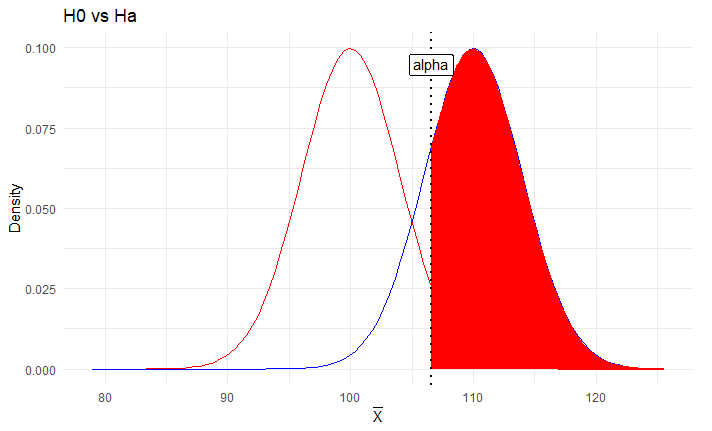
\includegraphics{plot_potencia.png}

Plot Two-Sample

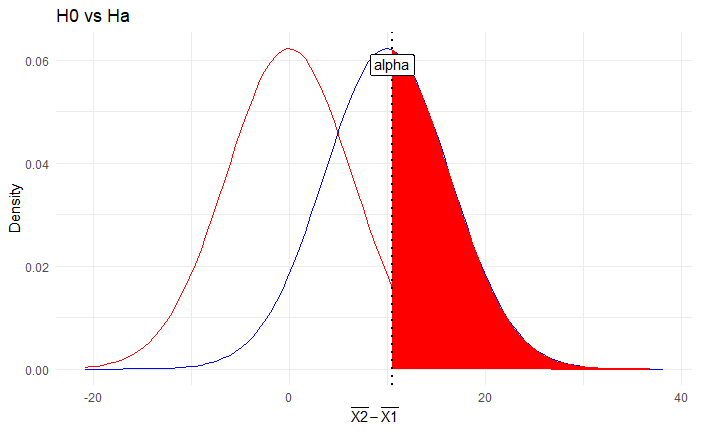
\includegraphics{plot_potencia_2.png}

Para los plots deberían obtener algo similar a las figuras expuestas,
donde en los plots se pueden ver las hipótesis que componen el test y el
área roja bajo la curva representa la potencia del test.

\begin{itemize}
\tightlist
\item
  Si utiliza el esqueleto propuesto, complete y comente que realiza cada
  una de las partes de la función one-sample entregada.
\end{itemize}

Codificada la función realice los siguientes experimentos:

\begin{itemize}
\tightlist
\item
  Obtener el gráfico de potencia al variar la media poblacional para los
  siguientes argumentos de entrada:
\end{itemize}

\[ n1=16, sigma1=16, mu.Ha=100 , mu.True=Variar, alfa=0.05 \]
\[ n1=16, sigma1=16, mu.Ha=100 , mu.True= Variar, alfa=0.01 \]
\[ n1=16, sigma1=16, mu.Ha=100 , mu.True= Variar, alfa=0.1 \]

Se le recomienda que la variación se realice a través de un \texttt{for}
y grafique las curvas dentro de un mismo gráfico para observar
potenciales diferencias entre ellas.

\begin{itemize}
\item
  Diseñe un experimento one-sample y visualice cómo se comportan las
  distribuciones normales de la hipótesis nula y la hipótesis
  alternativa al variar \(\alpha\).
\item
  Diseñe un experimento Two-sample y visualice cómo se comportan las
  distribuciones normales de la hipótesis nula y la hipótesis
  alternativa al variar \(\alpha\).
\end{itemize}

Para el diseño de experimentos y/o comprobación de sus métodos puede
serles útiles (no hay problema si decide utilizar los mismos ejemplos):

\begin{itemize}
\tightlist
\item
  one-sample:
  \href{https://online.stat.psu.edu/stat415/lesson/25/25.2}{Power
  Functions}
\item
  Two-Sample:
  \href{https://ytliu0.github.io/Stat_Med/power2.html}{Simple Power
  Calculation for Two-Sample Z Test}
\end{itemize}

\textbf{Respuesta}

\begin{Shaded}
\begin{Highlighting}[]
\FunctionTok{library}\NormalTok{(ggplot2)}
\CommentTok{\# Power Function, El esqueleto posee como ejemplo como obtener la potencia de un z{-}test one{-}sample.}
\CommentTok{\# Si utiliza este esqueleto deberá comentar la función que cumple cada una de las partes entregadas}
\NormalTok{power.z.test }\OtherTok{\textless{}{-}} \ControlFlowTok{function}\NormalTok{(}\AttributeTok{n1=}\ConstantTok{NULL}\NormalTok{, }\AttributeTok{sigma1=}\FloatTok{0.5}\NormalTok{, }
                         \AttributeTok{n2=}\ConstantTok{NULL}\NormalTok{,}\AttributeTok{sigma2=}\FloatTok{0.5}\NormalTok{, }\AttributeTok{mu.Ha=}\DecValTok{0}\NormalTok{ , }
                         \AttributeTok{mu.True=}\DecValTok{0}\NormalTok{, }\AttributeTok{alfa=}\FloatTok{0.05}\NormalTok{)\{}
\NormalTok{  Z }\OtherTok{=} \FunctionTok{qnorm}\NormalTok{(}\DecValTok{1}\SpecialCharTok{{-}}\NormalTok{alfa)}
  
  \ControlFlowTok{if}\NormalTok{(}\FunctionTok{is.null}\NormalTok{(n2))\{}
    \CommentTok{\# Se calcula el valor del test estadístico Z, para alpha, para ver cuándo rechazar el test de        hipotesis nula}
    
    
    \CommentTok{\#se obtiene el aproximado de la dev std de la poblacion (que termina siendo el de la muestra)}
\NormalTok{    denominador }\OtherTok{=}\NormalTok{ sigma1}\SpecialCharTok{/}\FunctionTok{sqrt}\NormalTok{(n1)}
    \CommentTok{\#se obtiene el valor para rechazar la hip nula en los datos}
\NormalTok{    X\_bar }\OtherTok{=}\NormalTok{ Z}\SpecialCharTok{*}\NormalTok{denominador }\SpecialCharTok{+}\NormalTok{ mu.Ha}
    
    \CommentTok{\# se obtiene la diferencia entre el valor de rechazo y el valor de la media}
\NormalTok{    numerador }\OtherTok{=}\NormalTok{ X\_bar }\SpecialCharTok{{-}}\NormalTok{ mu.True}
    
\NormalTok{    Z }\OtherTok{=}\NormalTok{ numerador}\SpecialCharTok{/}\NormalTok{denominador}
\NormalTok{    x\_label }\OtherTok{\textless{}{-}} \FunctionTok{expression}\NormalTok{(}\FunctionTok{bar}\NormalTok{(}\StringTok{"X"}\NormalTok{))}
    \CommentTok{\# se calcula la probabilidad de rechazar la hipotesis nula p = 1 {-} beta}
\NormalTok{    Power }\OtherTok{=} \DecValTok{1} \SpecialCharTok{{-}} \FunctionTok{pnorm}\NormalTok{(Z)}
    

\NormalTok{  \}}
  \ControlFlowTok{if}\NormalTok{(}\SpecialCharTok{!}\FunctionTok{is.null}\NormalTok{(n2))\{}
    
    \CommentTok{\#n1=NULL, sigma1=0.5,n2=NULL,sigma2=0.5, mu.Ha=0 , mu.True=0, alfa=0.05}
    \CommentTok{\# Calculamos el error estandar de ambas distribuciones}
\NormalTok{    denominador }\OtherTok{=} \FunctionTok{sqrt}\NormalTok{((sigma1}\SpecialCharTok{\^{}}\DecValTok{2}\NormalTok{)}\SpecialCharTok{/}\NormalTok{n1 }\SpecialCharTok{+}\NormalTok{ (sigma2}\SpecialCharTok{\^{}}\DecValTok{2}\NormalTok{)}\SpecialCharTok{/}\NormalTok{n2)}
    
    \CommentTok{\# mu.Ha representará la diferencia entre las medias de las muestras}
    \CommentTok{\# mu.True la diferencia de las medias de la población de las muestras 1 y 2.}
    
    \CommentTok{\# Z{-}score = mu.Ha / error standard}
\NormalTok{      Z\_score }\OtherTok{=}\NormalTok{ mu.Ha }\SpecialCharTok{/}\NormalTok{ denominador}
      
\NormalTok{      X\_bar }\OtherTok{=}\NormalTok{ Z}\SpecialCharTok{*}\NormalTok{denominador }\SpecialCharTok{+}\NormalTok{ mu.Ha}
      
\NormalTok{      Power }\OtherTok{=} \DecValTok{2}\SpecialCharTok{*}\FunctionTok{pnorm}\NormalTok{(}\SpecialCharTok{{-}}\FunctionTok{abs}\NormalTok{(Z\_score))}
    
\NormalTok{      x\_label }\OtherTok{\textless{}{-}} \FunctionTok{expression}\NormalTok{(}\FunctionTok{bar}\NormalTok{(X2) }\SpecialCharTok{{-}} \FunctionTok{bar}\NormalTok{(X1))}
    \CommentTok{\# }
\NormalTok{    plot }\OtherTok{=} \ConstantTok{NULL} \CommentTok{\# Solo esta null para que puedan ejecutarlo.}
  
\NormalTok{  \}}
    
    
        \CommentTok{\# Calculamos el mínimo y máximo de la distribucion normal con media mu.ha y sd = se}
\NormalTok{    min\_lim }\OtherTok{=} \FunctionTok{min}\NormalTok{(}\FunctionTok{rnorm}\NormalTok{(}\DecValTok{1000}\NormalTok{, }\AttributeTok{mean=}\NormalTok{mu.Ha, }\AttributeTok{sd=}\NormalTok{denominador)) }\SpecialCharTok{{-}} 
      \FunctionTok{round}\NormalTok{(}\FunctionTok{min}\NormalTok{(}\FunctionTok{rnorm}\NormalTok{(}\DecValTok{1000}\NormalTok{, }\AttributeTok{mean=}\NormalTok{mu.Ha, }\AttributeTok{sd=}\NormalTok{denominador)))}\SpecialCharTok{\%\%}\DecValTok{10}
\NormalTok{    max\_lim }\OtherTok{=} \FunctionTok{max}\NormalTok{(}\FunctionTok{rnorm}\NormalTok{(}\DecValTok{1000}\NormalTok{, }\AttributeTok{mean=}\NormalTok{mu.True, }\AttributeTok{sd=}\NormalTok{denominador)) }\SpecialCharTok{+}
      \FunctionTok{round}\NormalTok{(}\FunctionTok{max}\NormalTok{(}\FunctionTok{rnorm}\NormalTok{(}\DecValTok{1000}\NormalTok{, }\AttributeTok{mean=}\NormalTok{mu.True, }\AttributeTok{sd=}\NormalTok{denominador)))}\SpecialCharTok{\%\%}\DecValTok{10}
      
    \CommentTok{\# Generamos el plot con las curvas de la distribucion normal de la poblacion y la muestra}
\NormalTok{    plot }\OtherTok{\textless{}{-}} \FunctionTok{ggplot}\NormalTok{(}\FunctionTok{data.frame}\NormalTok{(}\AttributeTok{x =} \FunctionTok{c}\NormalTok{(min\_lim, max\_lim)), }\FunctionTok{aes}\NormalTok{(x)) }\SpecialCharTok{+} 
      \FunctionTok{stat\_function}\NormalTok{(}\AttributeTok{fun =}\NormalTok{ dnorm, }\AttributeTok{args =} \FunctionTok{list}\NormalTok{(}\AttributeTok{mean =}\NormalTok{ mu.Ha, }\AttributeTok{sd =}\NormalTok{ denominador), }
                    \AttributeTok{col=}\StringTok{\textquotesingle{}red\textquotesingle{}}\NormalTok{) }\SpecialCharTok{+}
      \FunctionTok{stat\_function}\NormalTok{(}\AttributeTok{fun =}\NormalTok{ dnorm, }\AttributeTok{args =} \FunctionTok{list}\NormalTok{(}\AttributeTok{mean =}\NormalTok{ mu.True, }\AttributeTok{sd =}\NormalTok{ denominador), }
                    \AttributeTok{col=}\StringTok{\textquotesingle{}blue\textquotesingle{}}\NormalTok{) }\SpecialCharTok{+}
      \FunctionTok{stat\_function}\NormalTok{(}\AttributeTok{fun =}\NormalTok{ dnorm, }\AttributeTok{args =} \FunctionTok{list}\NormalTok{(}\AttributeTok{mean =}\NormalTok{ mu.True, }\AttributeTok{sd =}\NormalTok{ denominador), }
                    \AttributeTok{xlim =} \FunctionTok{c}\NormalTok{(X\_bar,max\_lim), }\AttributeTok{geom =} \StringTok{"area"}\NormalTok{, }\AttributeTok{fill=}\StringTok{\textquotesingle{}red\textquotesingle{}}\NormalTok{) }\SpecialCharTok{+} 
      \FunctionTok{geom\_vline}\NormalTok{(}\AttributeTok{xintercept =}\NormalTok{ X\_bar, }\AttributeTok{linetype=}\StringTok{"dotted"}\NormalTok{, }\AttributeTok{size=}\DecValTok{1}\NormalTok{) }\SpecialCharTok{+}
      \FunctionTok{annotate}\NormalTok{(}\AttributeTok{x=}\NormalTok{X\_bar, }\AttributeTok{y=}\SpecialCharTok{+}\ConstantTok{Inf}\NormalTok{,}\AttributeTok{label=}\StringTok{"alpha"}\NormalTok{, }\AttributeTok{vjust=}\DecValTok{2}\NormalTok{, }\AttributeTok{geom=}\StringTok{"label"}\NormalTok{) }\SpecialCharTok{+}
      \FunctionTok{theme\_minimal}\NormalTok{() }\SpecialCharTok{+}
      \FunctionTok{ggtitle}\NormalTok{(}\StringTok{"H0 vs Ha"}\NormalTok{) }\SpecialCharTok{+}
      \FunctionTok{xlab}\NormalTok{(x\_label) }\SpecialCharTok{+}
      \FunctionTok{ylab}\NormalTok{(}\StringTok{"Density"}\NormalTok{)}

  \CommentTok{\# Como R no permite retornar dos salidas usamos una lista}
  \CommentTok{\# Los resultados se llaman con $plot o $power}
  \FunctionTok{return}\NormalTok{(}\FunctionTok{list}\NormalTok{(}\AttributeTok{plot=}\NormalTok{plot, }\AttributeTok{power=}\NormalTok{Power))}
\NormalTok{\}}
\end{Highlighting}
\end{Shaded}

\hypertarget{graficos-one-sample-usando-varios-ejemplos-modificando-alpha.-se-uso-y-modifico-ligeramente-el-esqueleto-de-ejemplo.}{%
\subsubsection{Gráficos one-sample usando varios ejemplos modificando
alpha. Se usó y modificó ligeramente el esqueleto de
ejemplo.}\label{graficos-one-sample-usando-varios-ejemplos-modificando-alpha.-se-uso-y-modifico-ligeramente-el-esqueleto-de-ejemplo.}}

\begin{Shaded}
\begin{Highlighting}[]
\NormalTok{one\_sided }\OtherTok{\textless{}{-}} \FunctionTok{power.z.test}\NormalTok{(}\AttributeTok{n1=}\DecValTok{16}\NormalTok{, }\AttributeTok{sigma1=}\DecValTok{16}\NormalTok{, }\AttributeTok{mu.True=}\DecValTok{8}\NormalTok{, }\AttributeTok{alfa=}\FloatTok{0.01}\NormalTok{)}
\NormalTok{one\_sided2 }\OtherTok{\textless{}{-}} \FunctionTok{power.z.test}\NormalTok{(}\AttributeTok{n1=}\DecValTok{16}\NormalTok{, }\AttributeTok{sigma1=}\DecValTok{16}\NormalTok{, }\AttributeTok{mu.True=}\DecValTok{8}\NormalTok{, }\AttributeTok{alfa=}\FloatTok{0.05}\NormalTok{)}
\NormalTok{one\_sided3 }\OtherTok{\textless{}{-}} \FunctionTok{power.z.test}\NormalTok{(}\AttributeTok{n1=}\DecValTok{16}\NormalTok{, }\AttributeTok{sigma1=}\DecValTok{16}\NormalTok{, }\AttributeTok{mu.True=}\DecValTok{8}\NormalTok{, }\AttributeTok{alfa=}\FloatTok{0.1}\NormalTok{)}
\FunctionTok{plot}\NormalTok{(one\_sided}\SpecialCharTok{$}\NormalTok{plot)}
\end{Highlighting}
\end{Shaded}

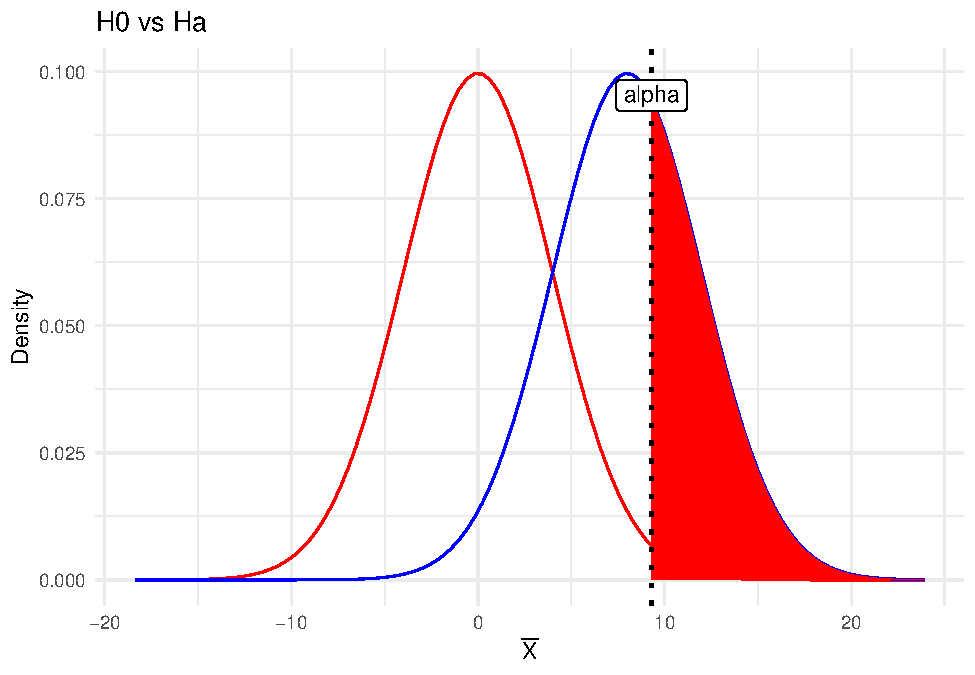
\includegraphics{Enunciado_Tarea_3_files/figure-latex/unnamed-chunk-3-1.pdf}

\begin{Shaded}
\begin{Highlighting}[]
\FunctionTok{plot}\NormalTok{(one\_sided2}\SpecialCharTok{$}\NormalTok{plot)}
\end{Highlighting}
\end{Shaded}

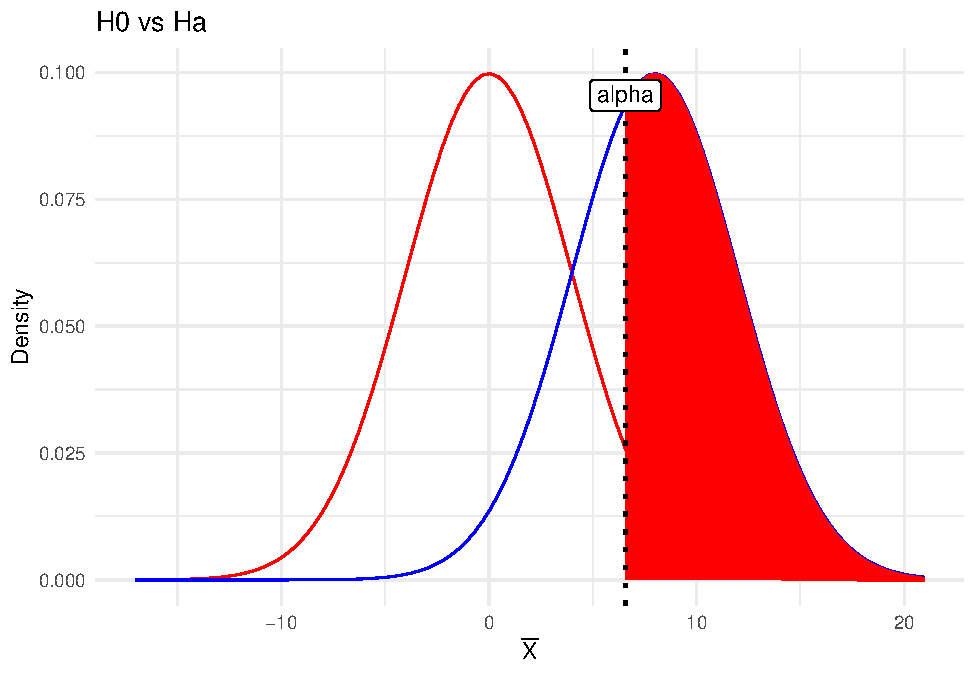
\includegraphics{Enunciado_Tarea_3_files/figure-latex/unnamed-chunk-3-2.pdf}

\begin{Shaded}
\begin{Highlighting}[]
\FunctionTok{plot}\NormalTok{(one\_sided3}\SpecialCharTok{$}\NormalTok{plot)}
\end{Highlighting}
\end{Shaded}

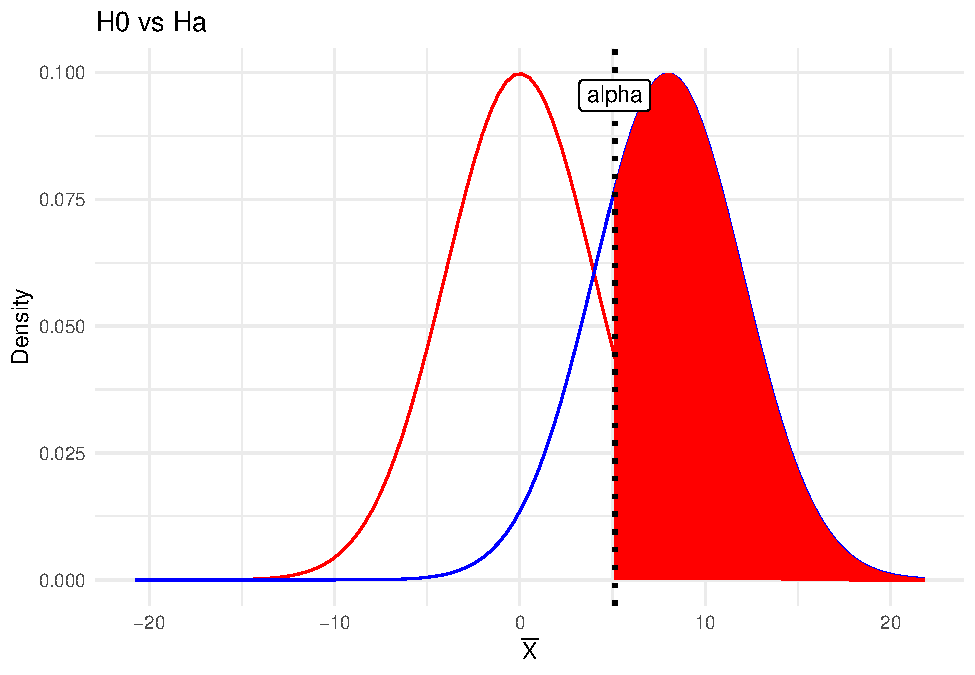
\includegraphics{Enunciado_Tarea_3_files/figure-latex/unnamed-chunk-3-3.pdf}

\hypertarget{graficos-two-sample-usando-varios-ejemplos-modificando-alpha.}{%
\subsubsection{Gráficos two-sample usando varios ejemplos modificando
alpha.}\label{graficos-two-sample-usando-varios-ejemplos-modificando-alpha.}}

\begin{Shaded}
\begin{Highlighting}[]
\NormalTok{two\_sided }\OtherTok{\textless{}{-}} \FunctionTok{power.z.test}\NormalTok{(}\AttributeTok{n1=}\DecValTok{16}\NormalTok{, }\AttributeTok{sigma1=}\DecValTok{16}\NormalTok{, }\AttributeTok{n2=}\DecValTok{40}\NormalTok{, }\AttributeTok{sigma2 =} \DecValTok{25}\NormalTok{, }\AttributeTok{mu.Ha=}\DecValTok{100}\NormalTok{ , }\AttributeTok{mu.True=}\DecValTok{110}\NormalTok{, }\AttributeTok{alfa=}\FloatTok{0.01}\NormalTok{)}
\NormalTok{two\_sided2 }\OtherTok{\textless{}{-}} \FunctionTok{power.z.test}\NormalTok{(}\AttributeTok{n1=}\DecValTok{16}\NormalTok{, }\AttributeTok{sigma1=}\DecValTok{16}\NormalTok{, }\AttributeTok{n2=}\DecValTok{40}\NormalTok{, }\AttributeTok{sigma2 =} \DecValTok{25}\NormalTok{, }\AttributeTok{mu.Ha=}\DecValTok{100}\NormalTok{ , }\AttributeTok{mu.True=}\DecValTok{110}\NormalTok{, }\AttributeTok{alfa=}\FloatTok{0.05}\NormalTok{)}
\NormalTok{two\_sided3 }\OtherTok{\textless{}{-}} \FunctionTok{power.z.test}\NormalTok{(}\AttributeTok{n1=}\DecValTok{16}\NormalTok{, }\AttributeTok{sigma1=}\DecValTok{16}\NormalTok{, }\AttributeTok{n2=}\DecValTok{40}\NormalTok{, }\AttributeTok{sigma2 =} \DecValTok{25}\NormalTok{, }\AttributeTok{mu.Ha=}\DecValTok{100}\NormalTok{ , }\AttributeTok{mu.True=}\DecValTok{110}\NormalTok{, }\AttributeTok{alfa=}\FloatTok{0.1}\NormalTok{)}
\FunctionTok{plot}\NormalTok{(two\_sided}\SpecialCharTok{$}\NormalTok{plot)}
\end{Highlighting}
\end{Shaded}

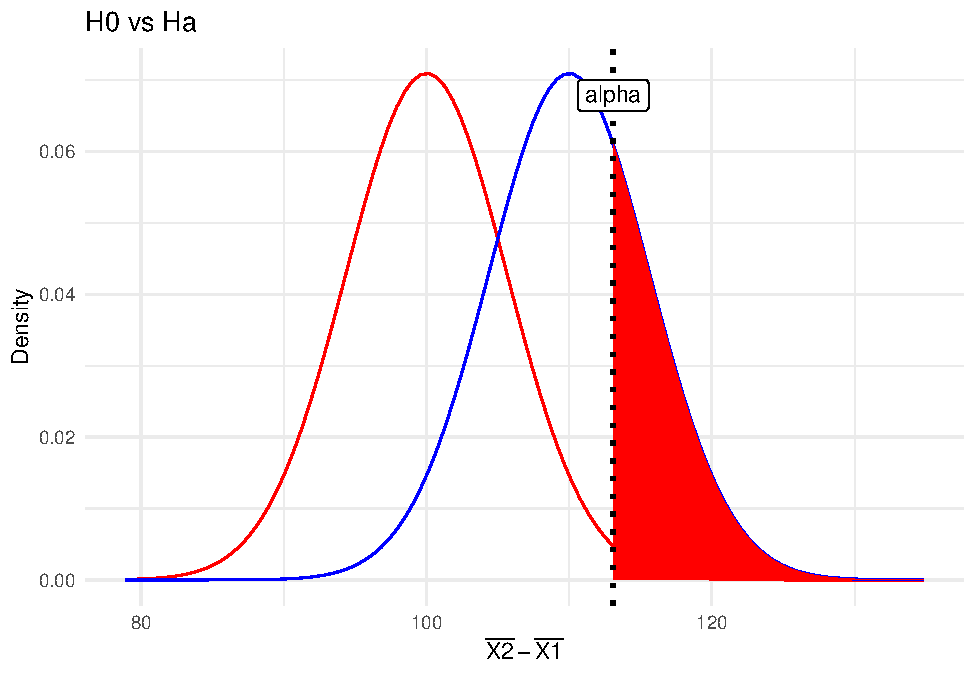
\includegraphics{Enunciado_Tarea_3_files/figure-latex/unnamed-chunk-4-1.pdf}

\begin{Shaded}
\begin{Highlighting}[]
\FunctionTok{plot}\NormalTok{(two\_sided2}\SpecialCharTok{$}\NormalTok{plot)}
\end{Highlighting}
\end{Shaded}

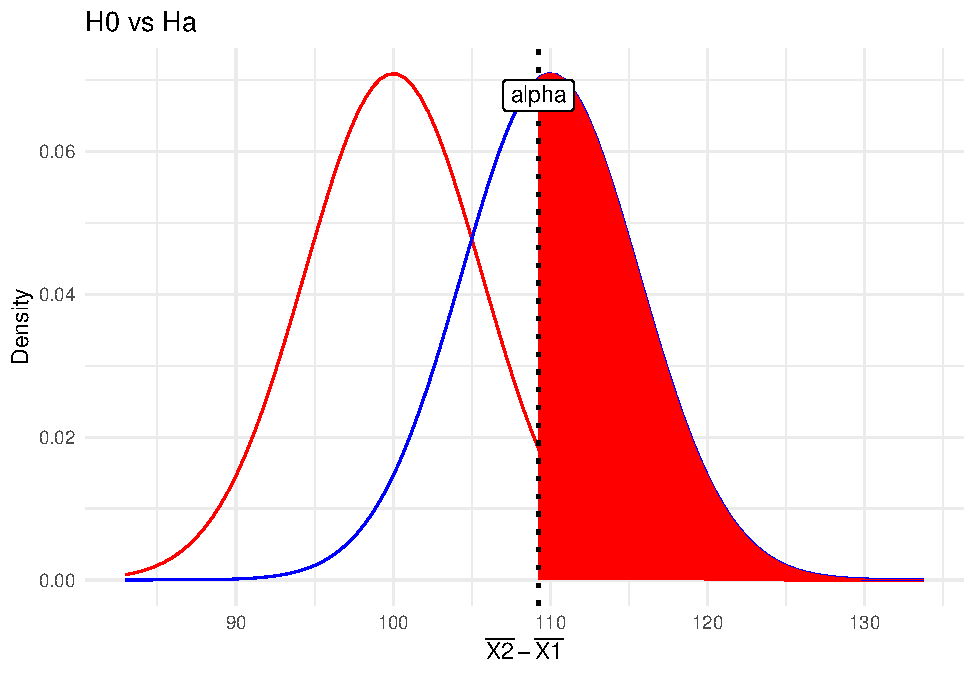
\includegraphics{Enunciado_Tarea_3_files/figure-latex/unnamed-chunk-4-2.pdf}

\begin{Shaded}
\begin{Highlighting}[]
\FunctionTok{plot}\NormalTok{(two\_sided3}\SpecialCharTok{$}\NormalTok{plot)}
\end{Highlighting}
\end{Shaded}

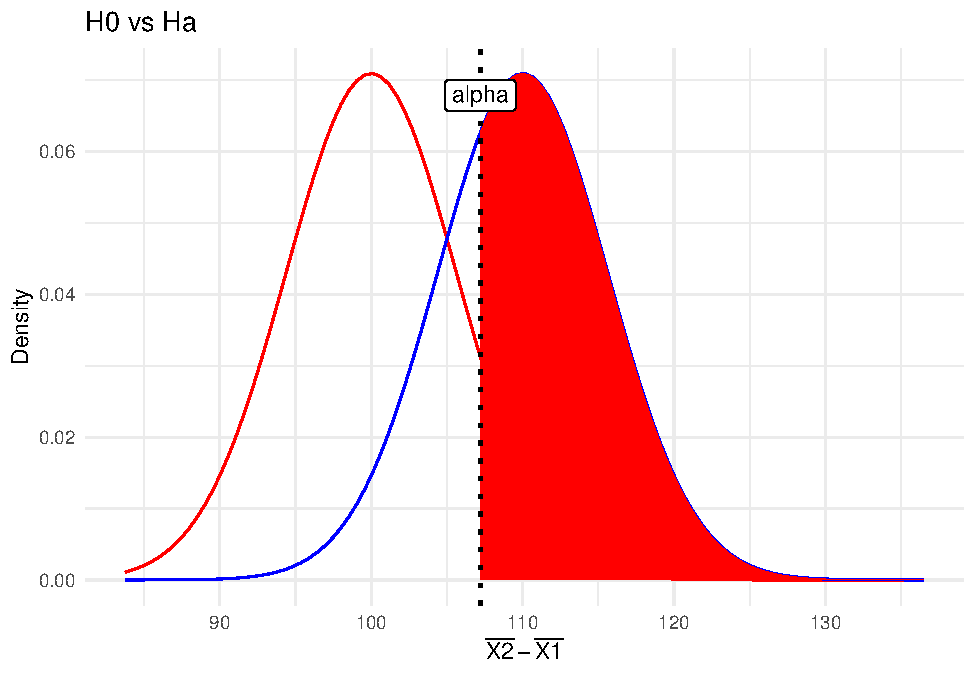
\includegraphics{Enunciado_Tarea_3_files/figure-latex/unnamed-chunk-4-3.pdf}

\hypertarget{experimentos-one_tail-variando-alfa-y-mu.ha-usando-el-esqueleto-propuesto.}{%
\subsection{\texorpdfstring{Experimentos one\_tail variando alfa y mu.Ha
\emph{usando el esqueleto
propuesto}.}{Experimentos one\_tail variando alfa y mu.Ha usando el esqueleto propuesto.}}\label{experimentos-one_tail-variando-alfa-y-mu.ha-usando-el-esqueleto-propuesto.}}

\begin{Shaded}
\begin{Highlighting}[]
\NormalTok{lista2 }\OtherTok{\textless{}{-}} \FunctionTok{c}\NormalTok{()}
\NormalTok{lista3 }\OtherTok{\textless{}{-}} \FunctionTok{c}\NormalTok{()}
\NormalTok{lista4 }\OtherTok{\textless{}{-}} \FunctionTok{c}\NormalTok{()}

\ControlFlowTok{for}\NormalTok{ (val }\ControlFlowTok{in} \FunctionTok{c}\NormalTok{( }\DecValTok{85}\SpecialCharTok{:}\DecValTok{125}\NormalTok{))\{}
\NormalTok{  uw }\OtherTok{\textless{}{-}}  \FunctionTok{power.z.test}\NormalTok{(}\AttributeTok{n1=}\DecValTok{16}\NormalTok{, }\AttributeTok{sigma1=}\DecValTok{16}\NormalTok{, }\AttributeTok{mu.Ha=}\DecValTok{100}\NormalTok{ , }\AttributeTok{mu.True=}\NormalTok{val, }\AttributeTok{alfa=}\FloatTok{0.01}\NormalTok{)}
\NormalTok{  uw1 }\OtherTok{\textless{}{-}} \FunctionTok{power.z.test}\NormalTok{(}\AttributeTok{n1=}\DecValTok{16}\NormalTok{, }\AttributeTok{sigma1=}\DecValTok{16}\NormalTok{, }\AttributeTok{mu.Ha=}\DecValTok{100}\NormalTok{ , }\AttributeTok{mu.True=}\NormalTok{val, }\AttributeTok{alfa=}\FloatTok{0.05}\NormalTok{)}
\NormalTok{  uw2 }\OtherTok{\textless{}{-}} \FunctionTok{power.z.test}\NormalTok{(}\AttributeTok{n1=}\DecValTok{16}\NormalTok{, }\AttributeTok{sigma1=}\DecValTok{16}\NormalTok{, }\AttributeTok{mu.Ha=}\DecValTok{100}\NormalTok{ , }\AttributeTok{mu.True=}\NormalTok{val, }\AttributeTok{alfa=}\FloatTok{0.1}\NormalTok{)}
\NormalTok{  lista2 }\OtherTok{\textless{}{-}} \FunctionTok{c}\NormalTok{(lista2, uw}\SpecialCharTok{$}\NormalTok{power)}
\NormalTok{  lista3 }\OtherTok{\textless{}{-}} \FunctionTok{c}\NormalTok{(lista3, uw1}\SpecialCharTok{$}\NormalTok{power)}
\NormalTok{  lista4 }\OtherTok{\textless{}{-}} \FunctionTok{c}\NormalTok{(lista4, uw2}\SpecialCharTok{$}\NormalTok{power)}
\NormalTok{\} }
\NormalTok{df\_lista }\OtherTok{\textless{}{-}} \FunctionTok{data.frame}\NormalTok{(}\AttributeTok{mu\_True =} \FunctionTok{c}\NormalTok{( }\DecValTok{85}\SpecialCharTok{:}\DecValTok{125}\NormalTok{), }
                       \AttributeTok{p\_value\_001 =}\NormalTok{ lista2, }
                       \AttributeTok{p\_value\_005 =}\NormalTok{ lista3, }
                       \AttributeTok{p\_value\_01 =}\NormalTok{ lista4)}

\FunctionTok{ggplot}\NormalTok{() }\SpecialCharTok{+} 
    \FunctionTok{geom\_line}\NormalTok{(}\AttributeTok{data=}\NormalTok{df\_lista, }\FunctionTok{aes}\NormalTok{(}\AttributeTok{x =}\NormalTok{ mu\_True, }\AttributeTok{y =}\NormalTok{ p\_value\_001, }\AttributeTok{color=}\StringTok{"0.01"}\NormalTok{),   }\AttributeTok{size=}\DecValTok{1}\NormalTok{) }\SpecialCharTok{+}
  \FunctionTok{geom\_line}\NormalTok{(}\AttributeTok{data=}\NormalTok{df\_lista, }\FunctionTok{aes}\NormalTok{(}\AttributeTok{x =}\NormalTok{ mu\_True, }\AttributeTok{y =}\NormalTok{ p\_value\_005, }\AttributeTok{color=}\StringTok{"0.05"}\NormalTok{), }\AttributeTok{size=}\DecValTok{1}\NormalTok{) }\SpecialCharTok{+}
  \FunctionTok{geom\_line}\NormalTok{(}\AttributeTok{data=}\NormalTok{df\_lista, }\FunctionTok{aes}\NormalTok{(}\AttributeTok{x =}\NormalTok{ mu\_True, }\AttributeTok{y =}\NormalTok{ p\_value\_01,  }\AttributeTok{color=}\StringTok{"0.1"}\NormalTok{),  }\AttributeTok{size=}\DecValTok{1}\NormalTok{) }\SpecialCharTok{+} 
  \FunctionTok{xlab}\NormalTok{(}\StringTok{"Diferencia de las medias de la población entre x1 y x2"}\NormalTok{) }\SpecialCharTok{+}
  \FunctionTok{ylab}\NormalTok{(}\StringTok{"p{-}value"}\NormalTok{) }\SpecialCharTok{+}
  \FunctionTok{scale\_color\_manual}\NormalTok{(}\AttributeTok{name =} \StringTok{"Alpha"}\NormalTok{, }\AttributeTok{values =} \FunctionTok{c}\NormalTok{(}\StringTok{"0.01"}\OtherTok{=} \StringTok{"red"}\NormalTok{, }\StringTok{"0.05"}\OtherTok{=} \StringTok{"green"}\NormalTok{, }\StringTok{"0.1"}\OtherTok{=} \StringTok{"blue"}\NormalTok{))}
\end{Highlighting}
\end{Shaded}

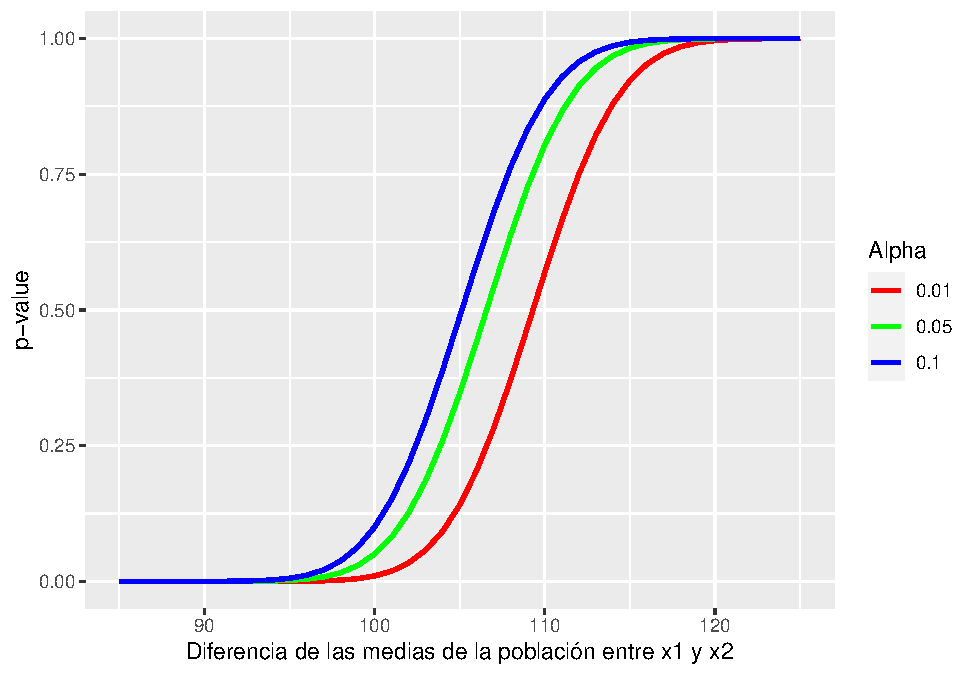
\includegraphics{Enunciado_Tarea_3_files/figure-latex/unnamed-chunk-5-1.pdf}

\begin{center}\rule{0.5\linewidth}{0.5pt}\end{center}

\hypertarget{pregunta-2-z-test}{%
\subsubsection{Pregunta 2: Z-test}\label{pregunta-2-z-test}}

Esta pregunta tiene como objetivo comprender como funciona un test de
hipótesis y como deberíamos abordar la realización de múltiples test de
hipótesis con datos reales.

La pregunta deberá ser desarrollada utilizando el dataset
\texttt{marketing\_campaign.csv}. Con esto, deberá programar un Z-test,
con el cual estudiará a través de experimentos el \texttt{Income} de
personas con los grados académicos \texttt{Graduation}, \texttt{Master}
y \texttt{PhD}. Para realizar esto considere la elaboración de los
siguientes puntos de forma secuencial:

\begin{itemize}
\tightlist
\item
  Modificar el dataframe entregado generando un estructura apta para el
  test de hipótesis. Una estructura que se les aconseja utilizar son
  vectores con los valores que representan a los grados académicos
  \texttt{Graduation}, \texttt{Master} y \texttt{PhD} por separado.
\end{itemize}

Ejemplo de estructura

Por ejemplo para el caso de Graduation pueden generar estructuras de la
siguiente forma:

\begin{longtable}[]{@{}ll@{}}
\toprule
ID & Graduation \\
\midrule
\endhead
5524 & 58138 \\
2174 & 46344 \\
4141 & 71613 \\
6182 & 26646 \\
965 & 55635 \\
\ldots{} & \ldots{} \\
\bottomrule
\end{longtable}

Donde los valores en la fila de Graduation representan los sueldos de
las diferentes personas que conforman el dataset. Un punto importante a
considerar es que los datos para los diferentes grados académicos poseen
diferentes numero de datos (no se asusten por esto).

\begin{itemize}
\item
  Programar el método Z-test con la metodología one sample y two sample,
  obteniendo los p-valores a través de las alternativas one-sided y
  two-sided. Para el caso de one-sided, cree una función capaz de
  obtener la cola menor y mayor de la gaussiana.
\item
  El calculo de las diferentes alternativas para calcular los p-valores
  deberá ser un argumento de su función, donde señalando `menor',`mayor'
  (para los casos one-sided) y `two-sided' deberá obtener el valor
  pertinente para cada caso.
\item
  Genere una función que permita realizar solo múltiples test del tipo
  two-sample y aplique bonferroni correction a los p-valores obtenidos.
  Notar que los múltiples test deberá realizar la comparación entre
  todos los elementos de entrada, por ejemplo si deseamos comparar los
  ingresos de \texttt{Graduation}, \texttt{Master} y \texttt{PhD}, se
  deberían comparar los ingresos de \texttt{Graduation} v/s
  \texttt{Master}, \texttt{Graduation} v/s \texttt{PhD} y
  \texttt{Master} y \texttt{PhD}
\end{itemize}

Codificada las funciones, realice los siguientes experimentos con su
función de test de hipótesis:

\begin{itemize}
\item
  Compruebe si la media de los ingresos para la variable
  \texttt{Graduation} es similar a 52000. Señale formalmente este
  experimento y obtenga los p-valores para las alternativas one-sided y
  two-sided.
\item
  Compruebe si la diferencia entre los ingresos de las personas con el
  grado académico \texttt{Graduation} es cercana a cero en relación a la
  recibida por los \texttt{Master} y \texttt{PhD}. Para este punto
  utilice la función que le permite realizar múltiples test del tipo
  two-sample.
\end{itemize}

Para los diferentes experimentos considere que la desviación estandar de
la población para los diferentes \texttt{income} son los siguientes:

\[\sigma_{Graduation} = 28180\] \[\sigma_{Master} = 20160\]
\[\sigma_{PhD} = 20615\]

\textbf{Respuesta:}

\begin{Shaded}
\begin{Highlighting}[]
\NormalTok{df }\OtherTok{=} \FunctionTok{read.csv}\NormalTok{(}\StringTok{\textquotesingle{}marketing\_campaign.csv\textquotesingle{}}\NormalTok{, }\AttributeTok{sep=}\StringTok{\textquotesingle{}}\SpecialCharTok{\textbackslash{}t}\StringTok{\textquotesingle{}}\NormalTok{)}

\CommentTok{\# Implementación de Z{-}test one{-}sided y two{-}sided}
\CommentTok{\# Puede utilizar este esqueleto}
\NormalTok{z\_test }\OtherTok{\textless{}{-}} \ControlFlowTok{function}\NormalTok{(}\AttributeTok{data1=}\ConstantTok{NULL}\NormalTok{, }\AttributeTok{sigma1=}\FloatTok{0.5}\NormalTok{, }\AttributeTok{data2=}\ConstantTok{NULL}\NormalTok{, }\AttributeTok{sigma2=}\FloatTok{0.5}\NormalTok{, }
                   \AttributeTok{mu.Ha=}\DecValTok{0}\NormalTok{, }\AttributeTok{test.type =} \FunctionTok{c}\NormalTok{(}\StringTok{\textquotesingle{}one{-}sided\textquotesingle{}}\NormalTok{,}\StringTok{\textquotesingle{}two{-}sided\textquotesingle{}}\NormalTok{),}
                   \AttributeTok{verbose=}\ConstantTok{TRUE}\NormalTok{)\{}
  
  \ControlFlowTok{if}\NormalTok{(}\FunctionTok{length}\NormalTok{(test.type)}\SpecialCharTok{\textgreater{}=}\DecValTok{2}\NormalTok{)\{}
    \FunctionTok{print}\NormalTok{(}\StringTok{"Por favor escoge un tipo de Test: ´one{-}sided´ o ´two{-}sided´ "}\NormalTok{)}
    \FunctionTok{return}\NormalTok{()}
\NormalTok{  \}}
  \ControlFlowTok{else} \ControlFlowTok{if}\NormalTok{(}\FunctionTok{length}\NormalTok{(test.type)}\SpecialCharTok{==}\DecValTok{1} \SpecialCharTok{\&\&} \SpecialCharTok{!}\NormalTok{(test.type }\SpecialCharTok{\%in\%} \FunctionTok{c}\NormalTok{(}\StringTok{\textquotesingle{}menor\textquotesingle{}}\NormalTok{,}\StringTok{\textquotesingle{}mayor\textquotesingle{}}\NormalTok{,}\StringTok{\textquotesingle{}two{-}sided\textquotesingle{}}\NormalTok{)))\{}
    \FunctionTok{print}\NormalTok{(}\StringTok{"Por favor escoge un tipo de Test: ´menor´, ´mayor´ o ´two{-}sided´"}\NormalTok{)}
    \FunctionTok{return}\NormalTok{()}
\NormalTok{  \}}
  \ControlFlowTok{else} \ControlFlowTok{if}\NormalTok{(}\FunctionTok{is.null}\NormalTok{(data2))\{}
\NormalTok{    mu\_1 }\OtherTok{=} \FunctionTok{mean}\NormalTok{(data1, }\AttributeTok{na.rm=}\ConstantTok{TRUE}\NormalTok{)}
\NormalTok{    n\_1 }\OtherTok{=} \FunctionTok{length}\NormalTok{(data1)}
\NormalTok{    Z\_score }\OtherTok{=}\NormalTok{ (mu\_1 }\SpecialCharTok{{-}}\NormalTok{ mu.Ha)}\SpecialCharTok{/}\NormalTok{(sigma1}\SpecialCharTok{/}\FunctionTok{sqrt}\NormalTok{(n\_1))}
    \CommentTok{\# P{-}value}
    \ControlFlowTok{if}\NormalTok{(test.type}\SpecialCharTok{==}\StringTok{\textquotesingle{}menor\textquotesingle{}}\NormalTok{)\{}
\NormalTok{      p\_value }\OtherTok{=} \FunctionTok{pnorm}\NormalTok{(Z\_score)}
\NormalTok{    \}}
    \ControlFlowTok{else} \ControlFlowTok{if}\NormalTok{(test.type}\SpecialCharTok{==}\StringTok{\textquotesingle{}mayor\textquotesingle{}}\NormalTok{)\{}
\NormalTok{      p\_value }\OtherTok{=} \DecValTok{1} \SpecialCharTok{{-}} \FunctionTok{pnorm}\NormalTok{(Z\_score)}
\NormalTok{    \}}
    \ControlFlowTok{else} \ControlFlowTok{if}\NormalTok{(test.type}\SpecialCharTok{==}\StringTok{\textquotesingle{}two{-}sided\textquotesingle{}}\NormalTok{)\{}
      \ControlFlowTok{if}\NormalTok{(mu\_1}\SpecialCharTok{\textgreater{}=}\NormalTok{mu.Ha)\{}
\NormalTok{        p\_value }\OtherTok{=}\NormalTok{ (}\DecValTok{1} \SpecialCharTok{{-}} \FunctionTok{pnorm}\NormalTok{(Z\_score))}\SpecialCharTok{*}\DecValTok{2}
\NormalTok{      \}}
      \ControlFlowTok{else} \ControlFlowTok{if}\NormalTok{(mu\_1}\SpecialCharTok{\textless{}}\NormalTok{mu.Ha)\{}
\NormalTok{        p\_value }\OtherTok{=}\NormalTok{ (}\FunctionTok{pnorm}\NormalTok{(Z\_score))}\SpecialCharTok{*}\DecValTok{2}
\NormalTok{      \}}
\NormalTok{    \}}
    \CommentTok{\# Texto de Salida}
    \ControlFlowTok{if}\NormalTok{(verbose)\{}
      \FunctionTok{cat}\NormalTok{(}\StringTok{"}\SpecialCharTok{\textbackslash{}t}\StringTok{One{-}sample Z{-}Test:}\SpecialCharTok{\textbackslash{}n\textbackslash{}n}\StringTok{Data analizada:"}\NormalTok{,}
                      \FunctionTok{deparse}\NormalTok{(}\FunctionTok{substitute}\NormalTok{(data1)), }\StringTok{"}\SpecialCharTok{\textbackslash{}n}\StringTok{Z="}\NormalTok{, Z\_score, }
                      \StringTok{"P{-}value="}\NormalTok{, p\_value, }\StringTok{"}\SpecialCharTok{\textbackslash{}n\textbackslash{}n}\StringTok{"}\NormalTok{,}\AttributeTok{sep=}\StringTok{" "}\NormalTok{)}
\NormalTok{    \}}
    
    \FunctionTok{return}\NormalTok{(p\_value)}
    
\NormalTok{  \}}
  \ControlFlowTok{else} \ControlFlowTok{if}\NormalTok{(}\SpecialCharTok{!}\FunctionTok{is.null}\NormalTok{(data2))\{}
    \CommentTok{\# Hypothesis test}
\NormalTok{    mu\_1 }\OtherTok{=} \FunctionTok{mean}\NormalTok{(data1, }\AttributeTok{na.rm=}\ConstantTok{TRUE}\NormalTok{)}
\NormalTok{    mu\_2 }\OtherTok{=} \FunctionTok{mean}\NormalTok{(data2, }\AttributeTok{na.rm=}\ConstantTok{TRUE}\NormalTok{)}
\NormalTok{    n\_1 }\OtherTok{=} \FunctionTok{length}\NormalTok{(data1)}
\NormalTok{    n\_2 }\OtherTok{=} \FunctionTok{length}\NormalTok{(data2)}
\NormalTok{    Z\_score }\OtherTok{=}\NormalTok{ (mu\_2 }\SpecialCharTok{{-}}\NormalTok{ mu\_1)}\SpecialCharTok{/}\FunctionTok{sqrt}\NormalTok{(((sigma1}\SpecialCharTok{\^{}}\DecValTok{2}\NormalTok{)}\SpecialCharTok{/}\NormalTok{n\_1 }\SpecialCharTok{+}\NormalTok{  (sigma2}\SpecialCharTok{\^{}}\DecValTok{2}\NormalTok{)}\SpecialCharTok{/}\NormalTok{n\_2))}
    \CommentTok{\# p{-}value}
    \ControlFlowTok{if}\NormalTok{(test.type}\SpecialCharTok{==}\StringTok{\textquotesingle{}menor\textquotesingle{}}\NormalTok{)\{}
\NormalTok{      p\_value }\OtherTok{=} \FunctionTok{pnorm}\NormalTok{(Z\_score)}
\NormalTok{    \}}
    \ControlFlowTok{else} \ControlFlowTok{if}\NormalTok{(test.type}\SpecialCharTok{==}\StringTok{\textquotesingle{}mayor\textquotesingle{}}\NormalTok{)\{}
\NormalTok{      p\_value }\OtherTok{=} \DecValTok{1} \SpecialCharTok{{-}} \FunctionTok{pnorm}\NormalTok{(Z\_score)}
\NormalTok{    \}}
    \ControlFlowTok{else} \ControlFlowTok{if}\NormalTok{(test.type}\SpecialCharTok{==}\StringTok{\textquotesingle{}two{-}sided\textquotesingle{}}\NormalTok{)\{}
      \ControlFlowTok{if}\NormalTok{(Z\_score}\SpecialCharTok{\textgreater{}=}\DecValTok{0}\NormalTok{)\{}
\NormalTok{        p\_value }\OtherTok{=}\NormalTok{ (}\DecValTok{1} \SpecialCharTok{{-}} \FunctionTok{pnorm}\NormalTok{(Z\_score))}\SpecialCharTok{*}\DecValTok{2}
\NormalTok{      \}}
      \ControlFlowTok{else} \ControlFlowTok{if}\NormalTok{(Z\_score}\SpecialCharTok{\textless{}}\DecValTok{0}\NormalTok{)\{}
\NormalTok{        p\_value }\OtherTok{=} \FunctionTok{pnorm}\NormalTok{(Z\_score)}\SpecialCharTok{*}\DecValTok{2}
\NormalTok{      \}}
\NormalTok{    \}}
    \CommentTok{\# Texto de Salida}
    \ControlFlowTok{if}\NormalTok{(verbose)\{}
      \FunctionTok{cat}\NormalTok{(}\StringTok{"}\SpecialCharTok{\textbackslash{}t}\StringTok{Two{-}sample Z{-}Test:}\SpecialCharTok{\textbackslash{}n\textbackslash{}n}\StringTok{Data analizada:"}\NormalTok{,}
                      \FunctionTok{deparse}\NormalTok{(}\FunctionTok{substitute}\NormalTok{(data1)),}\StringTok{"y"}\NormalTok{,}
                      \FunctionTok{deparse}\NormalTok{(}\FunctionTok{substitute}\NormalTok{(data2)), }\StringTok{"}\SpecialCharTok{\textbackslash{}n}\StringTok{Z="}\NormalTok{, }
\NormalTok{                      Z\_score, }\StringTok{"P{-}value="}\NormalTok{, p\_value, }\StringTok{"}\SpecialCharTok{\textbackslash{}n\textbackslash{}n}\StringTok{"}\NormalTok{,}\AttributeTok{sep=}\StringTok{" "}\NormalTok{)}
\NormalTok{    \}}
  
    \FunctionTok{return}\NormalTok{(p\_value)}
\NormalTok{  \}}
\NormalTok{\}}
\end{Highlighting}
\end{Shaded}

\begin{Shaded}
\begin{Highlighting}[]
\NormalTok{vec\_income\_PhD }\OtherTok{\textless{}{-}}\NormalTok{ df[df}\SpecialCharTok{$}\NormalTok{Education }\SpecialCharTok{==} \StringTok{\textquotesingle{}PhD\textquotesingle{}}\NormalTok{, ]}\SpecialCharTok{$}\NormalTok{Income}
\NormalTok{vec\_income\_Master }\OtherTok{\textless{}{-}}\NormalTok{ df[df}\SpecialCharTok{$}\NormalTok{Education }\SpecialCharTok{==} \StringTok{\textquotesingle{}Master\textquotesingle{}}\NormalTok{, ]}\SpecialCharTok{$}\NormalTok{Income}
\NormalTok{vec\_income\_Graduation }\OtherTok{\textless{}{-}}\NormalTok{ df[df}\SpecialCharTok{$}\NormalTok{Education }\SpecialCharTok{==} \StringTok{\textquotesingle{}Graduation\textquotesingle{}}\NormalTok{, ]}\SpecialCharTok{$}\NormalTok{Income}

\NormalTok{sigma\_PhD }\OtherTok{=} \DecValTok{20615}
\NormalTok{sigma\_Master }\OtherTok{=} \DecValTok{20160}
\NormalTok{sigma\_Graduation }\OtherTok{=} \DecValTok{28180}


\NormalTok{z.test.multiple\_testing }\OtherTok{\textless{}{-}} \ControlFlowTok{function}\NormalTok{()\{}
  \FunctionTok{print}\NormalTok{(}\StringTok{\textquotesingle{}Comprobar si la media de los ingresos para la variable Graduation es similar a 52000.\textquotesingle{}}\NormalTok{)}
\NormalTok{  p\_value\_1 }\OtherTok{=} \FunctionTok{z\_test}\NormalTok{(}\AttributeTok{data1=}\NormalTok{vec\_income\_Graduation, }\AttributeTok{sigma1=}\NormalTok{sigma\_Graduation, }\AttributeTok{mu.Ha=}\DecValTok{52000}\NormalTok{, }\AttributeTok{test.type=}\StringTok{\textquotesingle{}two{-}sided\textquotesingle{}}\NormalTok{, }\AttributeTok{verbose=}\ConstantTok{TRUE}\NormalTok{)}

  \FunctionTok{print}\NormalTok{(}\StringTok{\textquotesingle{}Compruebe si la diferencia entre los ingresos de las personas con el grado académico \textasciigrave{}Graduation\textasciigrave{} y \textasciigrave{}Master\textasciigrave{} es cercana a cero\textquotesingle{}}\NormalTok{)}
\NormalTok{  p\_value\_2 }\OtherTok{=} \FunctionTok{z\_test}\NormalTok{(}\AttributeTok{data1=}\NormalTok{vec\_income\_Graduation, }\AttributeTok{sigma1=}\NormalTok{sigma\_Graduation, }\AttributeTok{data2=}\NormalTok{vec\_income\_Master, }\AttributeTok{sigma2=}\NormalTok{sigma\_Master, }\AttributeTok{test.type=}\StringTok{\textquotesingle{}two{-}sided\textquotesingle{}}\NormalTok{, }\AttributeTok{verbose=}\ConstantTok{TRUE}\NormalTok{)}

  \FunctionTok{print}\NormalTok{(}\StringTok{\textquotesingle{}Compruebe si la diferencia entre los ingresos de las personas con el grado académico \textasciigrave{}Graduation\textasciigrave{} y \textasciigrave{}PhD\textasciigrave{} es cercana a cero\textquotesingle{}}\NormalTok{)}
\NormalTok{  p\_value\_3 }\OtherTok{=} \FunctionTok{z\_test}\NormalTok{(}\AttributeTok{data1=}\NormalTok{vec\_income\_Graduation, }\AttributeTok{sigma1=}\NormalTok{sigma\_Graduation, }\AttributeTok{data2=}\NormalTok{vec\_income\_PhD, }\AttributeTok{sigma2=}\NormalTok{sigma\_PhD, }\AttributeTok{test.type=}\StringTok{\textquotesingle{}two{-}sided\textquotesingle{}}\NormalTok{, }\AttributeTok{verbose=}\ConstantTok{TRUE}\NormalTok{)}
\NormalTok{\}}
\end{Highlighting}
\end{Shaded}

\textbf{Distribuciones}

Antes de hacer el test se muestran las curvas de ingresosos utilizadas,
esto con el fin de tener un mejor entendimiento de los resultados.
Además, visualizar los datos ayuda a corroborar el sentido de estos.

\begin{Shaded}
\begin{Highlighting}[]
\NormalTok{mean\_income\_PhD }\OtherTok{=} \FunctionTok{mean}\NormalTok{(vec\_income\_PhD, }\AttributeTok{na.rm=}\ConstantTok{TRUE}\NormalTok{)}
\NormalTok{mean\_income\_Master }\OtherTok{=} \FunctionTok{mean}\NormalTok{(vec\_income\_Master, }\AttributeTok{na.rm=}\ConstantTok{TRUE}\NormalTok{) }
\NormalTok{mean\_income\_Graduation }\OtherTok{=} \FunctionTok{mean}\NormalTok{(vec\_income\_Graduation, }\AttributeTok{na.rm=}\ConstantTok{TRUE}\NormalTok{)}

\NormalTok{length\_income\_PhD }\OtherTok{=} \FunctionTok{length}\NormalTok{(vec\_income\_PhD)}
\NormalTok{length\_income\_Master }\OtherTok{=} \FunctionTok{length}\NormalTok{(vec\_income\_Master) }
\NormalTok{length\_income\_Graduation }\OtherTok{=} \FunctionTok{length}\NormalTok{(vec\_income\_Graduation)}


\NormalTok{x }\OtherTok{\textless{}{-}} \FunctionTok{seq}\NormalTok{(}\DecValTok{0}\NormalTok{,}\DecValTok{140000}\NormalTok{,}\AttributeTok{length=}\DecValTok{1000}\NormalTok{)}
\FunctionTok{plot}\NormalTok{(x, }\FunctionTok{dnorm}\NormalTok{(x,}\AttributeTok{mean=}\NormalTok{mean\_income\_Graduation,}\AttributeTok{sd=}\NormalTok{sigma\_Graduation), }\AttributeTok{type =} \StringTok{"l"}\NormalTok{,}\AttributeTok{lty=}\DecValTok{1}\NormalTok{,}\AttributeTok{lwd=}\DecValTok{3}\NormalTok{, }\AttributeTok{col =} \StringTok{"blue"}\NormalTok{, }\AttributeTok{xlim=}\FunctionTok{c}\NormalTok{(}\DecValTok{0}\NormalTok{,}\DecValTok{140000}\NormalTok{), }\AttributeTok{ylim=}\FunctionTok{c}\NormalTok{(}\DecValTok{0}\NormalTok{,}\FloatTok{0.00003}\NormalTok{), }\AttributeTok{ylab =} \StringTok{"Probabilidad"}\NormalTok{, }\AttributeTok{xlab =} \StringTok{"Income"}\NormalTok{, }\AttributeTok{main=}\StringTok{"Distribuciones de sueldos según grado académico"}\NormalTok{)}
\FunctionTok{lines}\NormalTok{(x, }\FunctionTok{dnorm}\NormalTok{(x,}\AttributeTok{mean=}\NormalTok{mean\_income\_Master,}\AttributeTok{sd=}\NormalTok{sigma\_Master), }\AttributeTok{type =} \StringTok{"l"}\NormalTok{, }\AttributeTok{col =} \StringTok{"orange"}\NormalTok{)}
\FunctionTok{lines}\NormalTok{(x, }\FunctionTok{dnorm}\NormalTok{(x,}\AttributeTok{mean=}\NormalTok{mean\_income\_PhD,}\AttributeTok{sd=}\NormalTok{sigma\_PhD), }\AttributeTok{type =} \StringTok{"l"}\NormalTok{, }\AttributeTok{col =} \StringTok{"red"}\NormalTok{)}

\FunctionTok{legend}\NormalTok{(}\DecValTok{100000}\NormalTok{, }\FloatTok{0.00003}\NormalTok{, }\AttributeTok{legend=}\FunctionTok{c}\NormalTok{(}\StringTok{"Graduation"}\NormalTok{, }\StringTok{"Maste"}\NormalTok{, }\StringTok{"PhD"}\NormalTok{),}
       \AttributeTok{col=}\FunctionTok{c}\NormalTok{(}\StringTok{"blue"}\NormalTok{, }\StringTok{"orange"}\NormalTok{,}\StringTok{"red"}\NormalTok{), }\AttributeTok{lty=}\DecValTok{1}\SpecialCharTok{:}\DecValTok{2}\NormalTok{, }\AttributeTok{cex=}\FloatTok{0.8}\NormalTok{)}
\end{Highlighting}
\end{Shaded}

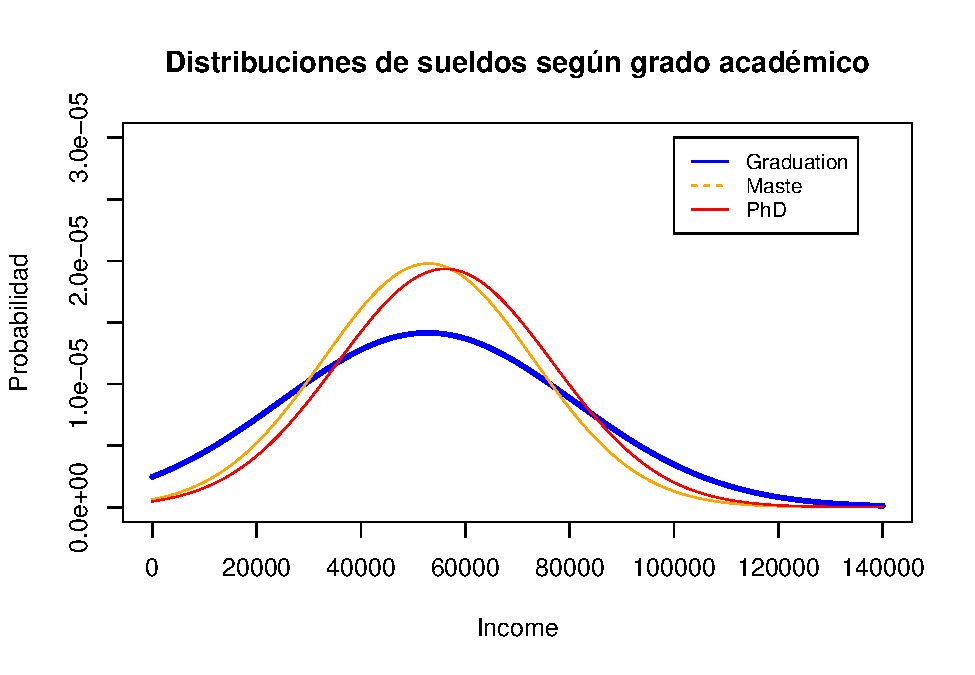
\includegraphics{Enunciado_Tarea_3_files/figure-latex/unnamed-chunk-8-1.pdf}

\textbf{Test} Se realiza el multitest definido anteriormente.

\begin{Shaded}
\begin{Highlighting}[]
\FunctionTok{z.test.multiple\_testing}\NormalTok{()}
\end{Highlighting}
\end{Shaded}

\begin{verbatim}
## [1] "Comprobar si la media de los ingresos para la variable Graduation es similar a 52000."
##  One-sample Z-Test:
## 
## Data analizada: vec_income_Graduation 
## Z= 0.8581808 P-value= 0.3907926 
## 
## [1] "Compruebe si la diferencia entre los ingresos de las personas con el grado académico `Graduation` y `Master` es cercana a cero"
##  Two-sample Z-Test:
## 
## Data analizada: vec_income_Graduation y vec_income_Master 
## Z= 0.1468296 P-value= 0.8832666 
## 
## [1] "Compruebe si la diferencia entre los ingresos de las personas con el grado académico `Graduation` y `PhD` es cercana a cero"
##  Two-sample Z-Test:
## 
## Data analizada: vec_income_Graduation y vec_income_PhD 
## Z= 2.725542 P-value= 0.0064196
\end{verbatim}

Como resputado del test se tienen los siguientes resultados

\begin{itemize}
\tightlist
\item
  Se rechaza que los valores estén distanciados. Se concluye que la
  variable Graduation es similar a 52000.
\item
  Se rechaza que los valores estén distanciados. Se concluye que la
  variable Graduation es similar a la variable Magister.
\item
  Se acepta que los valores están distnaciados. Se concluye que la
  variable Graduation es diferente a la variable PhD.
\end{itemize}

\hypertarget{pregunta-3-testeando-multiples-hipotesis-y-bonferroni-correction}{%
\subsubsection{Pregunta 3: Testeando multiples hipotesis y Bonferroni
Correction}\label{pregunta-3-testeando-multiples-hipotesis-y-bonferroni-correction}}

El objetivo de este problema es estudiar como realizar múltiples test de
hipótesis simultáneamente. Para esto en primer lugar se estudiara el
método ``intuitivo'', donde veremos sus limitantes y se comparará con el
método llamado \textbf{Bonferroni correction}, posteriormente se
realizará un estudio practico con el dataset \texttt{ratones.csv}.

Un investigador se ha colocado en contacto con ustedes señalándoles que
realiza diariamente test de hipótesis entre las muestras que toma día a
día en su laboratorio. Con esto, al investigador le urge saber si
realizar multiples test de hipótesis sin una corrección podría afectar
la toma de decisiones. Para comprobar esto, les solicita comprobar
matemáticamente como se comporta la probabilidad de obtener al menos un
resultado significativos al azar de sus experimentos diarios. Para esto,
les señala que la la probabilidad de obtener un experimento por azar
puede ser simulado a través de los casos exitosos de una binomial
(valores mayores a cero), donde el numero de observaciones son la
cantidad de experimentos (\(m\)) y la probabilidad queda dada por
\(\alpha\) del test.

A continuación, se entregan unas indicaciones mas especificas para
desarrollar la pregunta:

\begin{itemize}
\tightlist
\item[$\square$]
  Complete el código presentado a continuación que le permite calcular
  la probabilidad empírica de que obtenga al menos un resultado
  significativo para significancia \(\alpha\) y cantidad de experimentos
  \(m\) arbitrarios.
\item[$\square$]
  Se puede verificar que para un nivel de significancia \(\alpha\) y
  \(m\) experimentos independientes la probabilidad de que se tenga al
  menos un resultado significativo por azar es
  \[\mathbb{P}(\text{obtener al menos resultado significativo por azar})=1-(1-\alpha)^{m}\]
\item[$\square$]
  Considere \(\alpha = 0.05\), grafique la probabilidad empírica y real
  variando el valor de \(m\) ¿Se parecen sus resultados? ¿Que sucede
  cuando la cantidad de experimentos crece mucho? ¿Este comportamiento
  depende del valor de significancia \(\alpha\)? ¿Es útil este método
  para la realización de múltiples test de hipótesis?
\item[$\square$]
  Para solucionar los inconvenientes del método anterior es posible
  utilizar el método de \textbf{Bonferroni correction}, modifique su
  código anterior para verificar lo anterior ¿Mejoran los resultados?
  ¿cual podría ser un problema si es que \(m\) es muy grande?
\item[$\square$]
  Ejecute el siguiente código que calcula el \(p\)-valor usual y el
  \(p\)-valor asociado a Bonferroni (que corresponde al \(p\)-valor * m
  donde \(m\) es el numero de experimentos), ¿Cuantos valores que
  originalmente se hubieran aceptado fueron rechazados si
  \(\alpha = 0.05\)? ¿Que implica esto sobre el nivel de falsos
  negativos de este metodo?
\end{itemize}

\begin{Shaded}
\begin{Highlighting}[]
\NormalTok{data }\OtherTok{\textless{}{-}} \FunctionTok{read.csv}\NormalTok{(}\StringTok{"ratones.csv"}\NormalTok{,}\AttributeTok{sep=} \StringTok{";"}\NormalTok{, }\AttributeTok{stringsAsFactors =}\NormalTok{ T)}
\NormalTok{data}\SpecialCharTok{$}\NormalTok{p.value }\OtherTok{\textless{}{-}} \FunctionTok{sub}\NormalTok{(}\StringTok{","}\NormalTok{,}\StringTok{"."}\NormalTok{,data}\SpecialCharTok{$}\NormalTok{p.value)}
\NormalTok{data}\SpecialCharTok{$}\NormalTok{p.value }\OtherTok{\textless{}{-}} \FunctionTok{as.numeric}\NormalTok{(data}\SpecialCharTok{$}\NormalTok{p.value)}
\NormalTok{data}\SpecialCharTok{$}\NormalTok{p.value.Bonferroni }\OtherTok{\textless{}{-}} \FunctionTok{sub}\NormalTok{(}\StringTok{","}\NormalTok{,}\StringTok{"."}\NormalTok{,data}\SpecialCharTok{$}\NormalTok{p.value.Bonferroni)}
\NormalTok{data}\SpecialCharTok{$}\NormalTok{p.value.Bonferroni }\OtherTok{\textless{}{-}} \FunctionTok{as.numeric}\NormalTok{(data}\SpecialCharTok{$}\NormalTok{p.value.Bonferroni)}
\FunctionTok{head}\NormalTok{(data)}
\end{Highlighting}
\end{Shaded}

\begin{verbatim}
##   ï..Grupo.Ratones    p.value p.value.Bonferroni
## 1      NK603-11%+R 0.18797769           1.000000
## 2        NK602-13% 0.00994600           0.228758
## 3      NK603-11%+R 0.51508635           1.000000
## 4      NK603-22%+R 0.28493944           1.000000
## 5        RoundUp B 0.08459162           1.000000
## 6        RoundUp A 0.97688776           1.000000
\end{verbatim}

\textbf{Respuesta Aquí:}

A continuación se tiene la función para calcular la probabilidad
empírica de obtener un resultado signifiativo. Esta probabilidad depende
del umbral del p valor (\(\alpha\)), el número de muestras (m), el
número de experimentos (n) y el tipo de p valor utilizado (normal o
Bonferroni).

\begin{Shaded}
\begin{Highlighting}[]
\NormalTok{probEmpirica }\OtherTok{\textless{}{-}} \ControlFlowTok{function}\NormalTok{(alpha,m,}\AttributeTok{n=}\DecValTok{100}\NormalTok{, }\AttributeTok{Bonferroni =} \ConstantTok{FALSE}\NormalTok{)\{}
  \ControlFlowTok{if}\NormalTok{ (Bonferroni)\{}
\NormalTok{    res }\OtherTok{=} \FunctionTok{c}\NormalTok{(data}\SpecialCharTok{$}\NormalTok{p.value.Bonferroni) }\CommentTok{\#Resultados de los experimentos}
\NormalTok{  \}}
  \ControlFlowTok{else}\NormalTok{\{}
\NormalTok{    res }\OtherTok{=} \FunctionTok{c}\NormalTok{(data}\SpecialCharTok{$}\NormalTok{p.value) }\CommentTok{\#Resultados de los experimentos}
\NormalTok{  \}}
  
  \CommentTok{\# Puede agergar todo el codigo que estime conveniente para calcular la probabilidad empirica}
\NormalTok{  values }\OtherTok{\textless{}{-}} \FunctionTok{vector}\NormalTok{()}
  \ControlFlowTok{for}\NormalTok{ (i }\ControlFlowTok{in} \DecValTok{1}\SpecialCharTok{:}\NormalTok{n)\{}
\NormalTok{    muestra }\OtherTok{=} \FunctionTok{sample}\NormalTok{(res, }\AttributeTok{size =}\NormalTok{ m, }\AttributeTok{replace =}\NormalTok{ T)}
\NormalTok{    values[i] }\OtherTok{=} \FunctionTok{any}\NormalTok{(alpha}\SpecialCharTok{\textgreater{}=}\NormalTok{muestra)}
\NormalTok{  \}}

\NormalTok{  prob }\OtherTok{\textless{}{-}}\FunctionTok{sum}\NormalTok{(values)}\SpecialCharTok{/}\NormalTok{n }\CommentTok{\# Probabilidad empirica}
  
  \FunctionTok{return}\NormalTok{(prob)}
\NormalTok{\}}
\end{Highlighting}
\end{Shaded}

A continuación se muestran los gráficos obtenidos de las distintas
pruebas.

\textbf{P valor}

\begin{Shaded}
\begin{Highlighting}[]
\ControlFlowTok{for}\NormalTok{ (n }\ControlFlowTok{in} \FunctionTok{c}\NormalTok{(}\DecValTok{10}\NormalTok{,}\DecValTok{100}\NormalTok{,}\DecValTok{1000}\NormalTok{))\{}
\NormalTok{  largo\_del\_dataset }\OtherTok{=} \FunctionTok{length}\NormalTok{(data}\SpecialCharTok{$}\NormalTok{p.value)}
\NormalTok{  prob\_estimada }\OtherTok{\textless{}{-}} \FunctionTok{c}\NormalTok{(}\DecValTok{1}\SpecialCharTok{:}\NormalTok{largo\_del\_dataset)}
\NormalTok{  prob\_real }\OtherTok{\textless{}{-}} \FunctionTok{c}\NormalTok{(}\DecValTok{1}\SpecialCharTok{:}\NormalTok{largo\_del\_dataset)}
\NormalTok{  alpha }\OtherTok{=} \FloatTok{0.05}
  \ControlFlowTok{for}\NormalTok{ (m }\ControlFlowTok{in} \DecValTok{1}\SpecialCharTok{:}\NormalTok{largo\_del\_dataset)\{}
\NormalTok{    prob\_estimada[m] }\OtherTok{=} \DecValTok{1}\SpecialCharTok{{-}}\NormalTok{(}\DecValTok{1}\SpecialCharTok{{-}}\NormalTok{alpha)}\SpecialCharTok{\^{}}\NormalTok{m}
\NormalTok{    prob\_real[m] }\OtherTok{=} \FunctionTok{probEmpirica}\NormalTok{(alpha,m,n)}
\NormalTok{  \}}
  \FunctionTok{plot}\NormalTok{(}\FunctionTok{c}\NormalTok{(}\DecValTok{1}\SpecialCharTok{:}\NormalTok{m), prob\_estimada, }\AttributeTok{type =} \StringTok{"l"}\NormalTok{, }\AttributeTok{col =} \StringTok{"blue"}\NormalTok{, }\AttributeTok{xlim=}\FunctionTok{c}\NormalTok{(}\DecValTok{1}\NormalTok{,m), }\AttributeTok{ylim=}\FunctionTok{c}\NormalTok{(}\DecValTok{0}\NormalTok{,}\DecValTok{1}\NormalTok{), }\AttributeTok{ylab =} \StringTok{"Probabilidad"}\NormalTok{, }\AttributeTok{xlab =} \StringTok{"Número de muestras"}\NormalTok{, }\AttributeTok{main=}
         \FunctionTok{paste}\NormalTok{(}\StringTok{"Probabilidad de obtener un resultado significatívo, N = "}\NormalTok{,n))}
  \FunctionTok{lines}\NormalTok{(}\FunctionTok{c}\NormalTok{(}\DecValTok{1}\SpecialCharTok{:}\NormalTok{m), prob\_real, }\AttributeTok{type =} \StringTok{"l"}\NormalTok{, }\AttributeTok{col =} \StringTok{"orange"}\NormalTok{)}
  \FunctionTok{legend}\NormalTok{(}\DecValTok{16}\NormalTok{, }\FloatTok{0.2}\NormalTok{, }\AttributeTok{legend=}\FunctionTok{c}\NormalTok{(}\StringTok{"Probabilidad estimada"}\NormalTok{, }\StringTok{"Probabilidad real"}\NormalTok{),}
         \AttributeTok{col=}\FunctionTok{c}\NormalTok{(}\StringTok{"blue"}\NormalTok{, }\StringTok{"orange"}\NormalTok{), }\AttributeTok{lty=}\DecValTok{1}\SpecialCharTok{:}\DecValTok{2}\NormalTok{, }\AttributeTok{cex=}\FloatTok{0.8}\NormalTok{)}
\NormalTok{\}}
\end{Highlighting}
\end{Shaded}

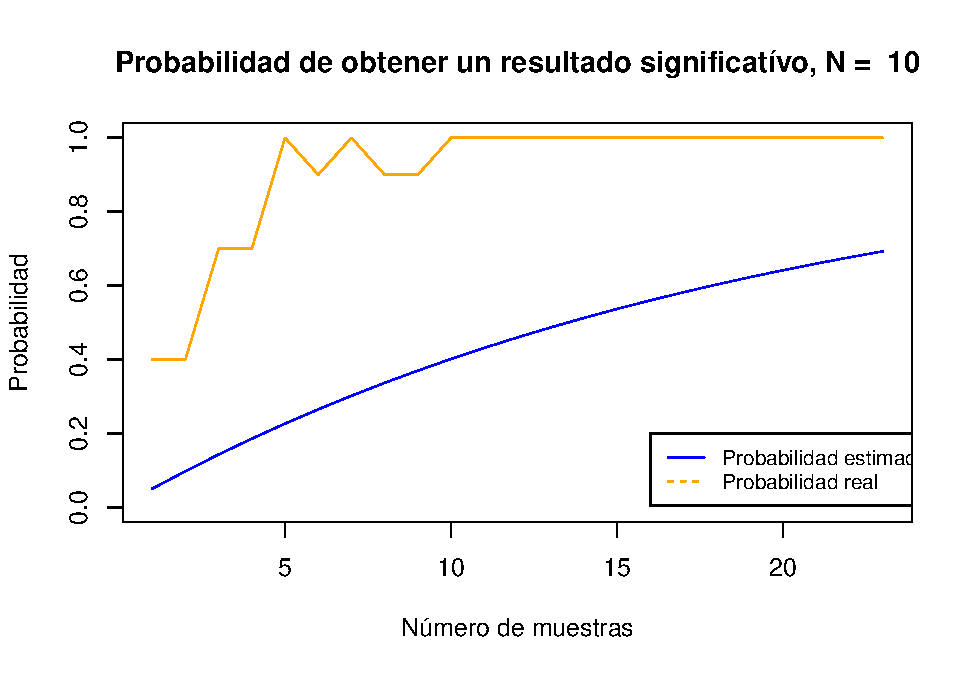
\includegraphics{Enunciado_Tarea_3_files/figure-latex/unnamed-chunk-12-1.pdf}
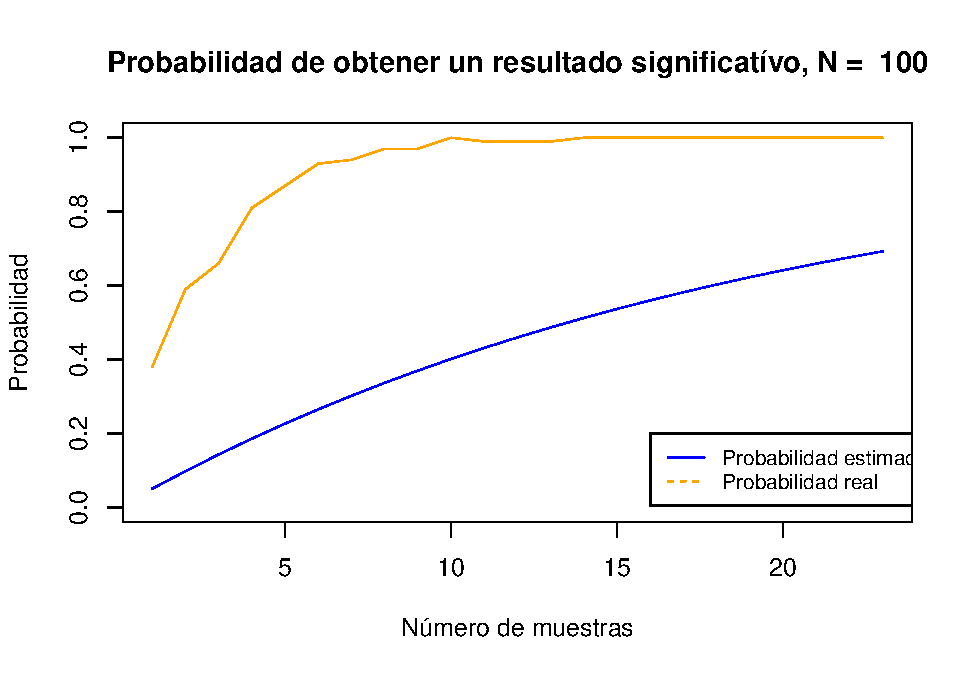
\includegraphics{Enunciado_Tarea_3_files/figure-latex/unnamed-chunk-12-2.pdf}
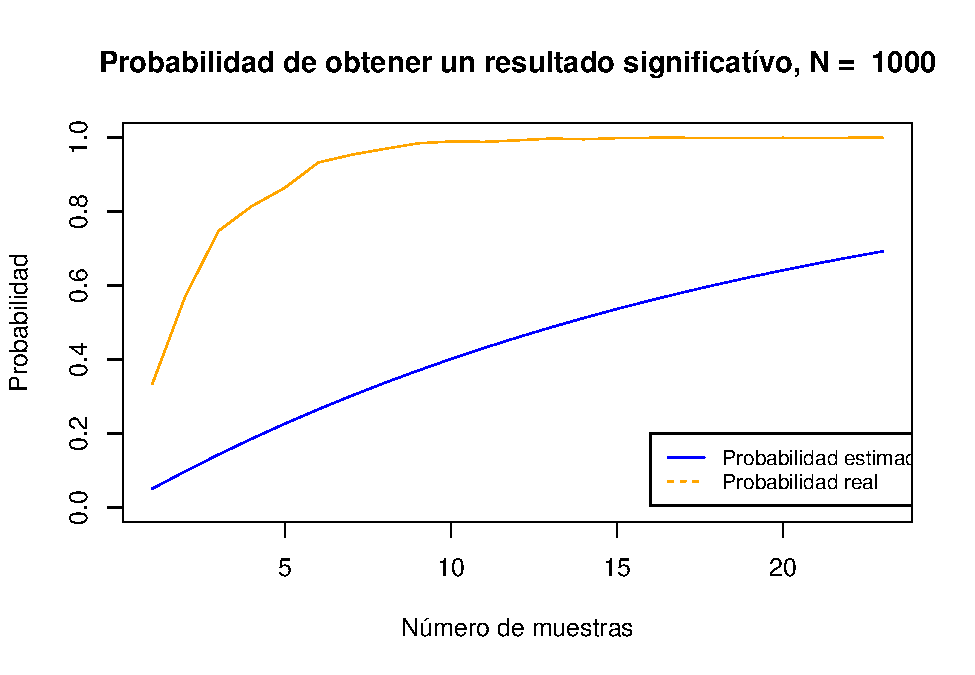
\includegraphics{Enunciado_Tarea_3_files/figure-latex/unnamed-chunk-12-3.pdf}

¿Se parecen sus resultados?

\begin{quote}
Ambas son crecientes pero no se parecen mucho, la probabilidad empírica
es mayor, alcanzando su límite mucho antes.
\end{quote}

¿Que sucede cuando la cantidad de experimentos crece mucho?

\begin{quote}
La unica curva que cambia con la cantidad de experimentos (n) es la
probabilidad empirica. Su curva se suavisa, esto porque converge a
probabilidades dado la ley de los grandes números. A medida que aumenta
el número de muestras (m) la probabilidad aumenta, lo cual tiene sentido
porque aumenta la oportunidad de obtener un resultado significativo.
\end{quote}

¿Este comportamiento depende del valor de significancia \(\alpha\)?

\begin{quote}
El resultado empírico si depende del valor de \(\alpha\), pero la forma
de la curva sigue siendo similar.
\end{quote}

¿Es útil este método para la realización de múltiples test de hipótesis?

\begin{quote}
Si es útil, pero la gran desventaja se aprecia en que la curva empírica
no coincide con la curva teórica. Podría ser mejor.
\end{quote}

\textbf{P valor Bonferroni}

\begin{Shaded}
\begin{Highlighting}[]
\ControlFlowTok{for}\NormalTok{ (n }\ControlFlowTok{in} \FunctionTok{c}\NormalTok{(}\DecValTok{10}\NormalTok{,}\DecValTok{100}\NormalTok{,}\DecValTok{1000}\NormalTok{))\{}
\NormalTok{  largo\_del\_dataset }\OtherTok{=} \FunctionTok{length}\NormalTok{(data}\SpecialCharTok{$}\NormalTok{p.value)}
\NormalTok{  prob\_estimada }\OtherTok{\textless{}{-}} \FunctionTok{c}\NormalTok{(}\DecValTok{1}\SpecialCharTok{:}\NormalTok{largo\_del\_dataset)}
\NormalTok{  prob\_real }\OtherTok{\textless{}{-}} \FunctionTok{c}\NormalTok{(}\DecValTok{1}\SpecialCharTok{:}\NormalTok{largo\_del\_dataset)}
\NormalTok{  alpha }\OtherTok{=} \FloatTok{0.05}
  \ControlFlowTok{for}\NormalTok{ (m }\ControlFlowTok{in} \DecValTok{1}\SpecialCharTok{:}\NormalTok{largo\_del\_dataset)\{}
\NormalTok{    prob\_estimada[m] }\OtherTok{=} \DecValTok{1}\SpecialCharTok{{-}}\NormalTok{(}\DecValTok{1}\SpecialCharTok{{-}}\NormalTok{alpha)}\SpecialCharTok{\^{}}\NormalTok{m}
\NormalTok{    prob\_real[m] }\OtherTok{=} \FunctionTok{probEmpirica}\NormalTok{(alpha,m,n, }\AttributeTok{Bonferroni =} \ConstantTok{TRUE}\NormalTok{)}
\NormalTok{  \}}
  \FunctionTok{plot}\NormalTok{(}\FunctionTok{c}\NormalTok{(}\DecValTok{1}\SpecialCharTok{:}\NormalTok{m), prob\_estimada, }\AttributeTok{type =} \StringTok{"l"}\NormalTok{, }\AttributeTok{col =} \StringTok{"blue"}\NormalTok{, }\AttributeTok{xlim=}\FunctionTok{c}\NormalTok{(}\DecValTok{1}\NormalTok{,m), }\AttributeTok{ylim=}\FunctionTok{c}\NormalTok{(}\DecValTok{0}\NormalTok{,}\DecValTok{1}\NormalTok{), }\AttributeTok{ylab =} \StringTok{"Probabilidad"}\NormalTok{, }\AttributeTok{xlab =} \StringTok{"Número de muestras"}\NormalTok{, }\AttributeTok{main=}
         \FunctionTok{paste}\NormalTok{(}\StringTok{"Probabilidad de obtener un resultado significatívo, N = "}\NormalTok{,n))}
  \FunctionTok{lines}\NormalTok{(}\FunctionTok{c}\NormalTok{(}\DecValTok{1}\SpecialCharTok{:}\NormalTok{m), prob\_real, }\AttributeTok{type =} \StringTok{"l"}\NormalTok{, }\AttributeTok{col =} \StringTok{"orange"}\NormalTok{)}
  \FunctionTok{legend}\NormalTok{(}\DecValTok{16}\NormalTok{, }\FloatTok{0.2}\NormalTok{, }\AttributeTok{legend=}\FunctionTok{c}\NormalTok{(}\StringTok{"Probabilidad estimada"}\NormalTok{, }\StringTok{"Probabilidad real"}\NormalTok{),}
         \AttributeTok{col=}\FunctionTok{c}\NormalTok{(}\StringTok{"blue"}\NormalTok{, }\StringTok{"orange"}\NormalTok{), }\AttributeTok{lty=}\DecValTok{1}\SpecialCharTok{:}\DecValTok{2}\NormalTok{, }\AttributeTok{cex=}\FloatTok{0.8}\NormalTok{)}
\NormalTok{\}}
\end{Highlighting}
\end{Shaded}

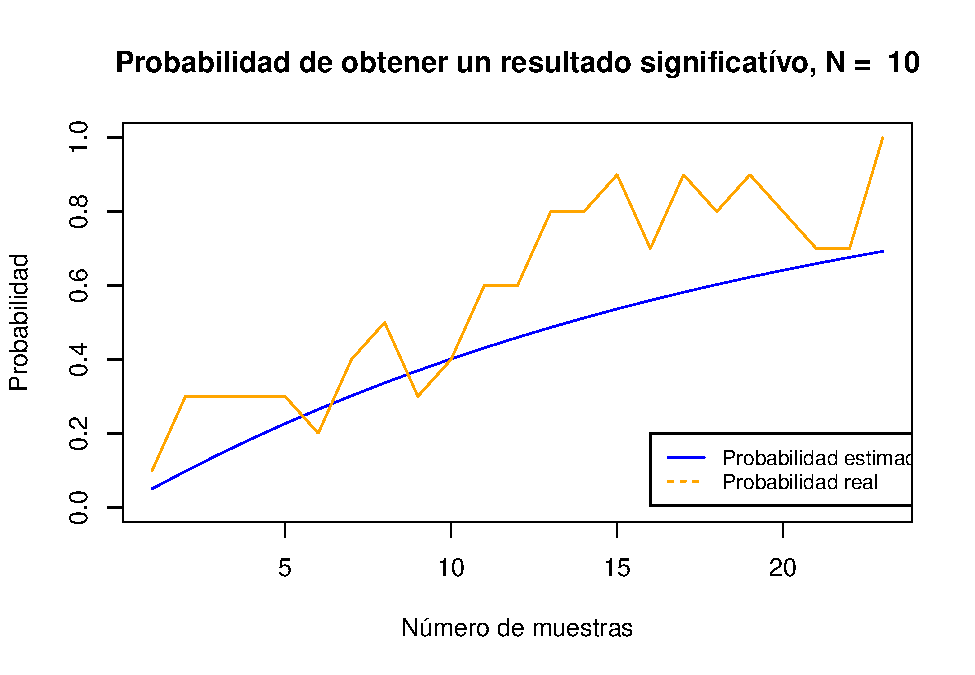
\includegraphics{Enunciado_Tarea_3_files/figure-latex/unnamed-chunk-13-1.pdf}
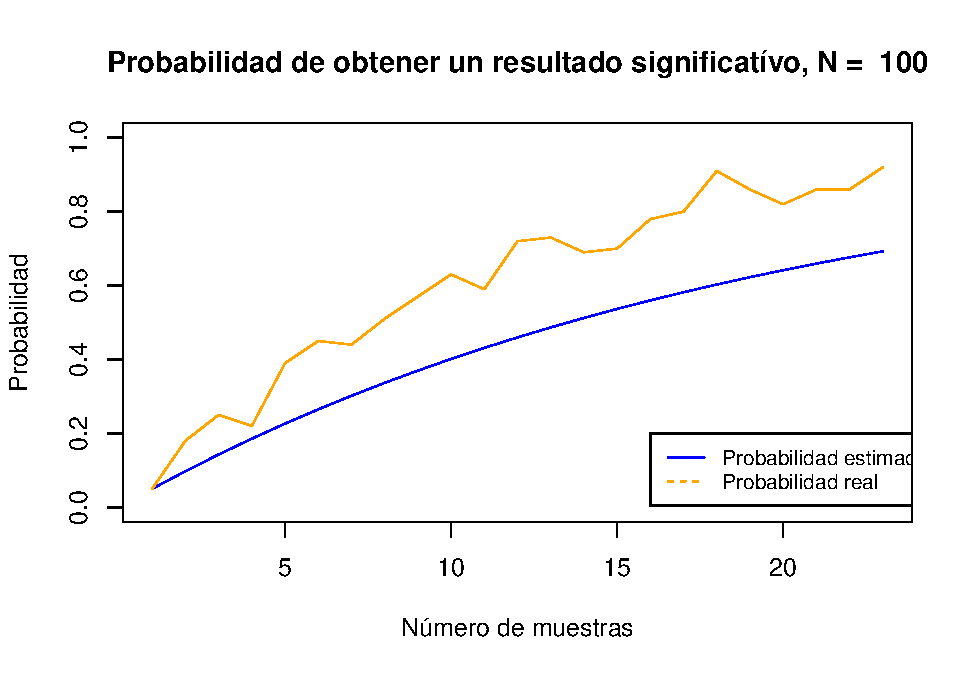
\includegraphics{Enunciado_Tarea_3_files/figure-latex/unnamed-chunk-13-2.pdf}
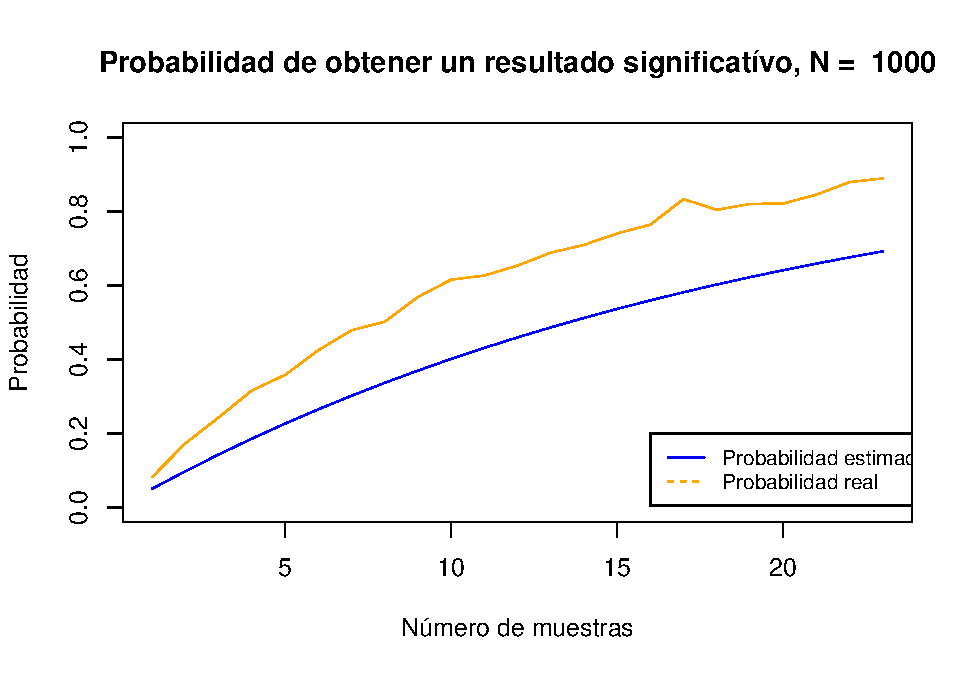
\includegraphics{Enunciado_Tarea_3_files/figure-latex/unnamed-chunk-13-3.pdf}

¿Mejoran los resultados?

\begin{quote}
Ahora los resultados empíricos son más cercanos a los estimados.
\end{quote}

¿Cual podría ser un problema si es que \(m\) es muy grande?

\begin{quote}
Al multiplicarse m por el p valor, un m grande puede reducir la
probabilidad de obtener resultados significativos. Un m muy grande puede
anular mucho la probabilidad de obtener resultados significativos, es
similar a disminuir \(\alpha\).
\end{quote}

\textbf{Preguntas generales} ¿Cuantos valores que originalmente se
hubieran aceptado fueron rechazados si \(\alpha = 0.05\)?

\begin{Shaded}
\begin{Highlighting}[]
\FunctionTok{print}\NormalTok{(}\FunctionTok{sum}\NormalTok{(alpha}\SpecialCharTok{\textgreater{}=}\NormalTok{data}\SpecialCharTok{$}\NormalTok{p.value))}
\end{Highlighting}
\end{Shaded}

\begin{verbatim}
## [1] 8
\end{verbatim}

\begin{Shaded}
\begin{Highlighting}[]
\FunctionTok{print}\NormalTok{(}\FunctionTok{sum}\NormalTok{(alpha}\SpecialCharTok{\textgreater{}=}\NormalTok{data}\SpecialCharTok{$}\NormalTok{p.value.Bonferroni))}
\end{Highlighting}
\end{Shaded}

\begin{verbatim}
## [1] 2
\end{verbatim}

\begin{quote}
Existen 6 valores que originalmente hubieran sido aceptados, pero con el
cambio no lo fueron.
\end{quote}

¿Que implica esto sobre el nivel de falsos negativos de este metodo?

\begin{quote}
Bajo la definicion de que un positivo corresponde a un resultado
significativo, esto implica un aumento en los falsos negativos. Esto se
puede ver en el ejemplo anterior, donde valores positivos se transforman
en valores negativos.
\end{quote}

\begin{center}\rule{0.5\linewidth}{0.5pt}\end{center}

\hypertarget{pregunta-4-regression-lineal-sin-comandos.}{%
\subsubsection{Pregunta 4: Regression Lineal sin
comandos.}\label{pregunta-4-regression-lineal-sin-comandos.}}

El objetivo de la siguiente pregunta es aplicar los conceptos de
regresión lineal vistos en clases para implementar desde cero un función
capaz de realizar una regresión simple y múltiple.

Para este problema, ustedes deberán estudiar el comportamiento de los
clientes de un holding de salud. Para esto, se les hace entrega del
dataset \texttt{insurance.csv} para que estudien la creación de un
modelo lineal con sus datos. Antes de comenzar a trabajar, se señalan
las diferentes variables que componen al dataset:

\begin{itemize}
\tightlist
\item
  age: Señala la edad de cada uno de los sujetos.
\item
  sex: Si es mujer es igual a 1, si es hombre es igual a 0.
\item
  bmi: Indice de masa corporal del cliente.
\item
  children: Señala cuantos hijos tiene cada uno de los sujetos.
\item
  smoker: Variable binaria que cuando es 1 señala que el cliente es
  fumador (0 en caso contrario).
\item
  charges: Gastos médicos de cada uno de los clientes.
\end{itemize}

Es importante que considere que cada una de las filas representa un
cliente distinto para el holding.

Dentro del estudio, el holding de salud le solicita estudiar los
comportamientos de los clientes fumadores y no fumadores, por lo que se
le aconseja separar el dataframe original en fumadores y no fumadores.
En el estudio, realicen un modelo lineal que tiene como variable de
respuesta a \texttt{charges} y los datos que mejor se correlacionan para
los clientes fumadores y no fumadores. Para esto, deberán realizar las
siguientes actividades:

\hypertarget{parte-i}{%
\paragraph{Parte I}\label{parte-i}}

\begin{enumerate}
\def\labelenumi{\alph{enumi})}
\tightlist
\item
  Programe un modelo lineal simple escogiendo la variable numérica que
  tiene mayor relación con la variable de respuesta. Recuerde justificar
  la elección de la variable numérica cuantitativamente.
\item
  Señale tanto el \(R^2\) como el \(R^2-adjustado\) del modelo.
\item
  Grafique el scatterplot de los datos y la linea que ajusta a la
  regresión lineal obtenida.
\end{enumerate}

\begin{Shaded}
\begin{Highlighting}[]
\FunctionTok{library}\NormalTok{(ggplot2)}
\FunctionTok{library}\NormalTok{(corrplot)}
\end{Highlighting}
\end{Shaded}

\begin{verbatim}
## corrplot 0.90 loaded
\end{verbatim}

\begin{Shaded}
\begin{Highlighting}[]
\NormalTok{my\_dat}\OtherTok{\textless{}{-}} \FunctionTok{read.csv}\NormalTok{(}\StringTok{\textquotesingle{}insurance.csv\textquotesingle{}}\NormalTok{, }\AttributeTok{header =} \ConstantTok{TRUE}\NormalTok{, }\AttributeTok{sep=} \StringTok{","}\NormalTok{, }\AttributeTok{quote =} \StringTok{\textquotesingle{}}\SpecialCharTok{\textbackslash{}"}\StringTok{\textquotesingle{}}\NormalTok{)}
\NormalTok{my\_dat }\OtherTok{\textless{}{-}}\NormalTok{  my\_dat[}\FunctionTok{c}\NormalTok{(}\DecValTok{1}\NormalTok{, }\DecValTok{3}\NormalTok{, }\DecValTok{4}\NormalTok{, }\DecValTok{5}\NormalTok{, }\DecValTok{7}\NormalTok{)]}

\NormalTok{fumadores    }\OtherTok{\textless{}{-}}\NormalTok{ my\_dat[my\_dat}\SpecialCharTok{$}\NormalTok{smoker }\SpecialCharTok{==} \StringTok{\textquotesingle{}yes\textquotesingle{}}\NormalTok{, ]}
\NormalTok{no\_fumadores }\OtherTok{\textless{}{-}}\NormalTok{ my\_dat[my\_dat}\SpecialCharTok{$}\NormalTok{smoker }\SpecialCharTok{==} \StringTok{\textquotesingle{}no\textquotesingle{}}\NormalTok{ , ]}

\FunctionTok{corrplot}\NormalTok{(}\FunctionTok{cor}\NormalTok{(fumadores[}\FunctionTok{c}\NormalTok{(}\DecValTok{1}\NormalTok{, }\DecValTok{2}\NormalTok{, }\DecValTok{3}\NormalTok{, }\DecValTok{5}\NormalTok{)]))}
\end{Highlighting}
\end{Shaded}

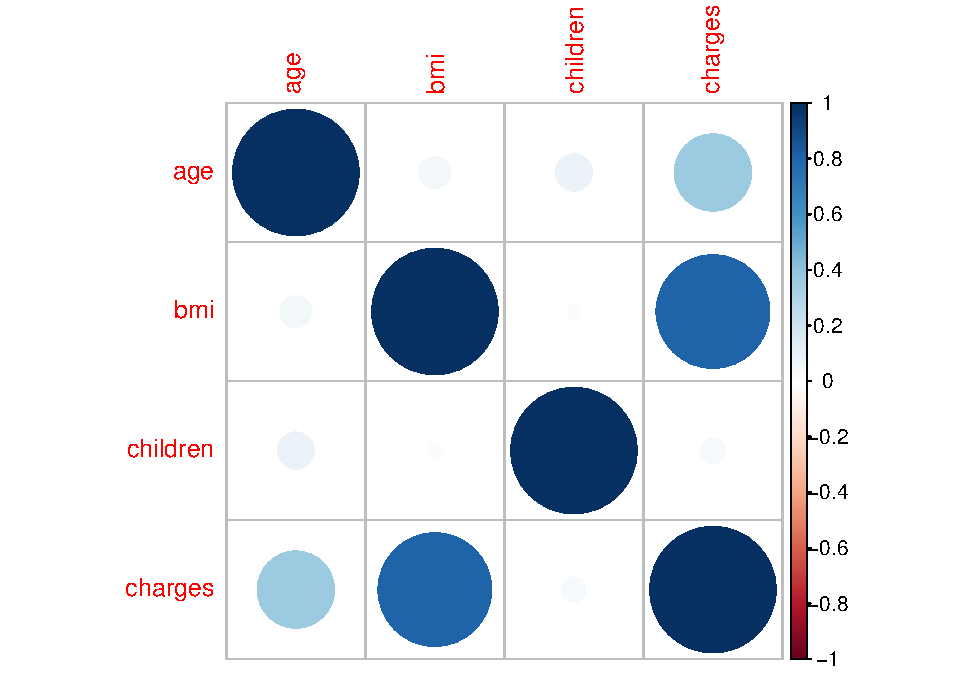
\includegraphics{Enunciado_Tarea_3_files/figure-latex/unnamed-chunk-15-1.pdf}

\begin{Shaded}
\begin{Highlighting}[]
\FunctionTok{corrplot}\NormalTok{(}\FunctionTok{cor}\NormalTok{(no\_fumadores[}\FunctionTok{c}\NormalTok{(}\DecValTok{1}\NormalTok{, }\DecValTok{2}\NormalTok{, }\DecValTok{3}\NormalTok{, }\DecValTok{5}\NormalTok{)]))}
\end{Highlighting}
\end{Shaded}

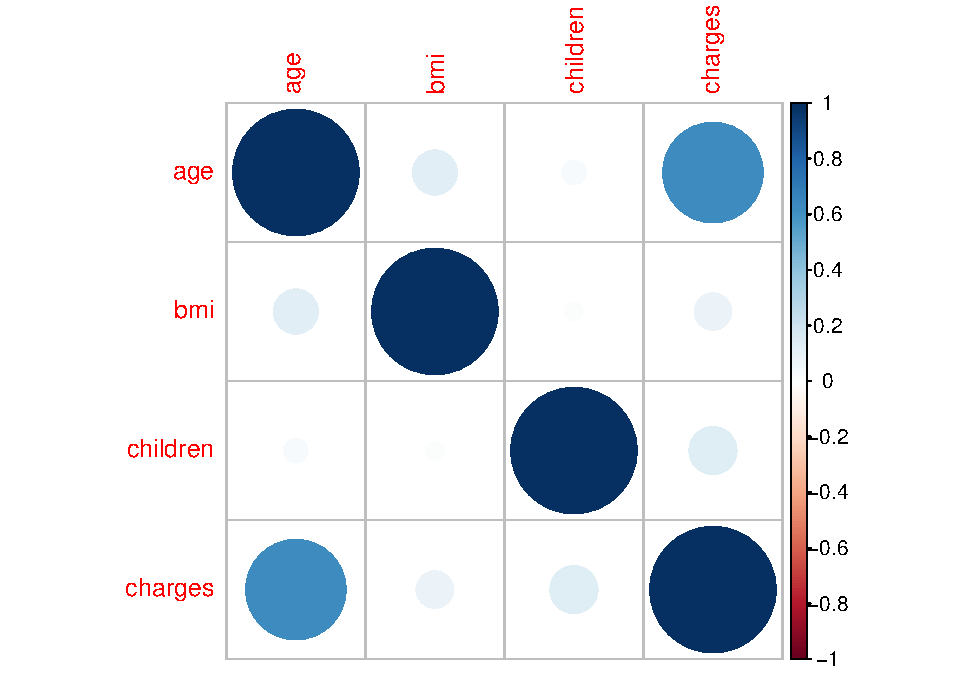
\includegraphics{Enunciado_Tarea_3_files/figure-latex/unnamed-chunk-15-2.pdf}
\#\# Análisis de los datos - Para fumadores: Podemos observar usando
herramientas como la correlación de Pearson que la mayor relación para
`charges' es con `bmi'. - Para no fumadores: Con el mismo método podemos
observar que la mayor relación para este grupo con `charges' es con
`age'.

Por lo anterior, para fumadores se utilizará la variable `bmi' y para no
fumadores la variable `age'.

\begin{Shaded}
\begin{Highlighting}[]
\NormalTok{mod\_lin\_funct }\OtherTok{\textless{}{-}} \ControlFlowTok{function}\NormalTok{(x, y)\{}
\NormalTok{  media\_x }\OtherTok{=} \FunctionTok{mean}\NormalTok{(x); media\_y }\OtherTok{=} \FunctionTok{mean}\NormalTok{(y)}
\NormalTok{  dif\_x }\OtherTok{\textless{}{-}}\NormalTok{ x }\SpecialCharTok{{-}}\NormalTok{ media\_x}
\NormalTok{  dif\_y }\OtherTok{\textless{}{-}}\NormalTok{ y }\SpecialCharTok{{-}}\NormalTok{ media\_y}
\NormalTok{  b\_1 }\OtherTok{\textless{}{-}} \FunctionTok{sum}\NormalTok{(dif\_x }\SpecialCharTok{*}\NormalTok{ dif\_y) }\SpecialCharTok{/} \FunctionTok{sum}\NormalTok{(dif\_x }\SpecialCharTok{\^{}} \DecValTok{2}\NormalTok{)}
\NormalTok{  b\_0 }\OtherTok{\textless{}{-}}\NormalTok{ media\_y }\SpecialCharTok{{-}}\NormalTok{ b\_1 }\SpecialCharTok{*}\NormalTok{ media\_x}
\NormalTok{  y\_gorro }\OtherTok{\textless{}{-}}\NormalTok{ b\_0 }\SpecialCharTok{+}\NormalTok{ x }\SpecialCharTok{*}\NormalTok{ b\_1}
\NormalTok{  SSM }\OtherTok{\textless{}{-}} \FunctionTok{sum}\NormalTok{((y\_gorro }\SpecialCharTok{{-}}\NormalTok{ media\_y)}\SpecialCharTok{\^{}}\DecValTok{2}\NormalTok{)}
\NormalTok{  SST }\OtherTok{\textless{}{-}} \FunctionTok{sum}\NormalTok{((y }\SpecialCharTok{{-}}\NormalTok{ media\_y)}\SpecialCharTok{\^{}}\DecValTok{2}\NormalTok{)}
  
\NormalTok{  r\_sqr }\OtherTok{\textless{}{-}}\NormalTok{ SSM }\SpecialCharTok{/}\NormalTok{ SST}
\NormalTok{  N }\OtherTok{=} \FunctionTok{length}\NormalTok{(x); k }\OtherTok{=} \DecValTok{1}
\NormalTok{  r\_sqr\_a }\OtherTok{\textless{}{-}} \DecValTok{1} \SpecialCharTok{{-}}\NormalTok{ ((N }\SpecialCharTok{{-}} \DecValTok{1}\NormalTok{)}\SpecialCharTok{/}\NormalTok{(N }\SpecialCharTok{{-}}\NormalTok{ k }\SpecialCharTok{{-}} \DecValTok{1}\NormalTok{))}\SpecialCharTok{*}\NormalTok{(}\DecValTok{1} \SpecialCharTok{{-}}\NormalTok{ r\_sqr)}
    
  \FunctionTok{data.frame}\NormalTok{(b\_0, b\_1, r\_sqr, r\_sqr\_a)}
\NormalTok{\}}

\NormalTok{fum\_age }\OtherTok{\textless{}{-}} \FunctionTok{mod\_lin\_funct}\NormalTok{(fumadores}\SpecialCharTok{$}\NormalTok{age, fumadores}\SpecialCharTok{$}\NormalTok{charges)}
\NormalTok{fum\_bmi }\OtherTok{\textless{}{-}} \FunctionTok{mod\_lin\_funct}\NormalTok{(fumadores}\SpecialCharTok{$}\NormalTok{bmi, fumadores}\SpecialCharTok{$}\NormalTok{charges)}
\NormalTok{fum\_children }\OtherTok{\textless{}{-}} \FunctionTok{mod\_lin\_funct}\NormalTok{(fumadores}\SpecialCharTok{$}\NormalTok{children, fumadores}\SpecialCharTok{$}\NormalTok{charges)}

\NormalTok{no\_fum\_age }\OtherTok{\textless{}{-}} \FunctionTok{mod\_lin\_funct}\NormalTok{(no\_fumadores}\SpecialCharTok{$}\NormalTok{age, no\_fumadores}\SpecialCharTok{$}\NormalTok{charges)}
\NormalTok{no\_fum\_bmi }\OtherTok{\textless{}{-}} \FunctionTok{mod\_lin\_funct}\NormalTok{(no\_fumadores}\SpecialCharTok{$}\NormalTok{bmi, no\_fumadores}\SpecialCharTok{$}\NormalTok{charges)}
\NormalTok{no\_fum\_children }\OtherTok{\textless{}{-}} \FunctionTok{mod\_lin\_funct}\NormalTok{(no\_fumadores}\SpecialCharTok{$}\NormalTok{children, no\_fumadores}\SpecialCharTok{$}\NormalTok{charges)}

\NormalTok{Tags }\OtherTok{\textless{}{-}} \FunctionTok{c}\NormalTok{(}\StringTok{"fum\_age"}\NormalTok{, }\StringTok{"fum\_bmi"}\NormalTok{, }\StringTok{"fum\_children"}\NormalTok{, }
          \StringTok{"no\_fum\_age"}\NormalTok{, }\StringTok{"no\_fum\_bmi"}\NormalTok{, }\StringTok{"no\_fum\_children"}\NormalTok{)}
\NormalTok{b\_0 }\OtherTok{\textless{}{-}} \FunctionTok{c}\NormalTok{(fum\_age}\SpecialCharTok{$}\NormalTok{b\_0, fum\_bmi}\SpecialCharTok{$}\NormalTok{b\_0, fum\_children}\SpecialCharTok{$}\NormalTok{b\_0, }
\NormalTok{         no\_fum\_age}\SpecialCharTok{$}\NormalTok{b\_0, no\_fum\_bmi}\SpecialCharTok{$}\NormalTok{b\_0, no\_fum\_children}\SpecialCharTok{$}\NormalTok{b\_0)}
\NormalTok{b\_1 }\OtherTok{\textless{}{-}}\FunctionTok{c}\NormalTok{(fum\_age}\SpecialCharTok{$}\NormalTok{b\_1, fum\_bmi}\SpecialCharTok{$}\NormalTok{b\_1, fum\_children}\SpecialCharTok{$}\NormalTok{b\_1, }
\NormalTok{         no\_fum\_age}\SpecialCharTok{$}\NormalTok{b\_1, no\_fum\_bmi}\SpecialCharTok{$}\NormalTok{b\_1, no\_fum\_children}\SpecialCharTok{$}\NormalTok{b\_1)}
\NormalTok{r\_sqr }\OtherTok{\textless{}{-}} \FunctionTok{c}\NormalTok{(fum\_age}\SpecialCharTok{$}\NormalTok{r\_sqr, fum\_bmi}\SpecialCharTok{$}\NormalTok{r\_sqr, fum\_children}\SpecialCharTok{$}\NormalTok{r\_sqr, }
\NormalTok{         no\_fum\_age}\SpecialCharTok{$}\NormalTok{r\_sqr, no\_fum\_bmi}\SpecialCharTok{$}\NormalTok{r\_sqr, no\_fum\_children}\SpecialCharTok{$}\NormalTok{r\_sqr)}
\NormalTok{r\_sqr\_a }\OtherTok{\textless{}{-}} \FunctionTok{c}\NormalTok{(fum\_age}\SpecialCharTok{$}\NormalTok{r\_sqr\_a, fum\_bmi}\SpecialCharTok{$}\NormalTok{r\_sqr\_a, fum\_children}\SpecialCharTok{$}\NormalTok{r\_sqr\_a, }
\NormalTok{         no\_fum\_age}\SpecialCharTok{$}\NormalTok{r\_sqr\_a, no\_fum\_bmi}\SpecialCharTok{$}\NormalTok{r\_sqr\_a, no\_fum\_children}\SpecialCharTok{$}\NormalTok{r\_sqr\_a)}
         
\NormalTok{resultados }\OtherTok{\textless{}{-}} \FunctionTok{data.frame}\NormalTok{(Tags, b\_0, b\_1, r\_sqr, r\_sqr\_a)}
\FunctionTok{print}\NormalTok{(resultados)}
\end{Highlighting}
\end{Shaded}

\begin{verbatim}
##              Tags        b_0        b_1       r_sqr      r_sqr_a
## 1         fum_age  20294.128  305.23760 0.135589241  0.132411260
## 2         fum_bmi -13186.576 1473.10625 0.650410969  0.649125716
## 3    fum_children  31651.121  358.54573 0.001292043 -0.002379677
## 4      no_fum_age  -2091.421  267.24891 0.394317163  0.393746840
## 5      no_fum_bmi   5879.424   83.35056 0.007062141  0.006127171
## 6 no_fum_children   7688.999  683.59223 0.019301185  0.018377740
\end{verbatim}

\hypertarget{resultados}{%
\subsection{Resultados}\label{resultados}}

A partir de estos datos, el modelo lineal para los fumadores consiste
en:
\[charges_{fumadores} = -13186 + 1473 * bmi,\,  R^2 = 0.650,\, R^2 \, ajustado = 0.649\]
Para los no fumadores:
\[charges_{no\_fumadores} = -2091 + 267 * age,\,  R^2 = 0.394,\, R^2 \, ajustado = 0.393\]

\begin{Shaded}
\begin{Highlighting}[]
\FunctionTok{ggplot}\NormalTok{(fumadores, }\FunctionTok{aes}\NormalTok{(}\AttributeTok{x=}\NormalTok{bmi, }\AttributeTok{y=}\NormalTok{charges)) }\SpecialCharTok{+}
  \FunctionTok{geom\_point}\NormalTok{(}\AttributeTok{size=}\DecValTok{2}\NormalTok{, }\AttributeTok{shape=}\DecValTok{23}\NormalTok{) }\SpecialCharTok{+}
  \FunctionTok{geom\_line}\NormalTok{(}\AttributeTok{y =}\NormalTok{ (fum\_bmi[}\DecValTok{1}\NormalTok{, }\DecValTok{1}\NormalTok{] }\SpecialCharTok{+} \FunctionTok{sort}\NormalTok{(fumadores}\SpecialCharTok{$}\NormalTok{bmi) }\SpecialCharTok{*}\NormalTok{ fum\_bmi[}\DecValTok{1}\NormalTok{, }\DecValTok{2}\NormalTok{]))}
\end{Highlighting}
\end{Shaded}

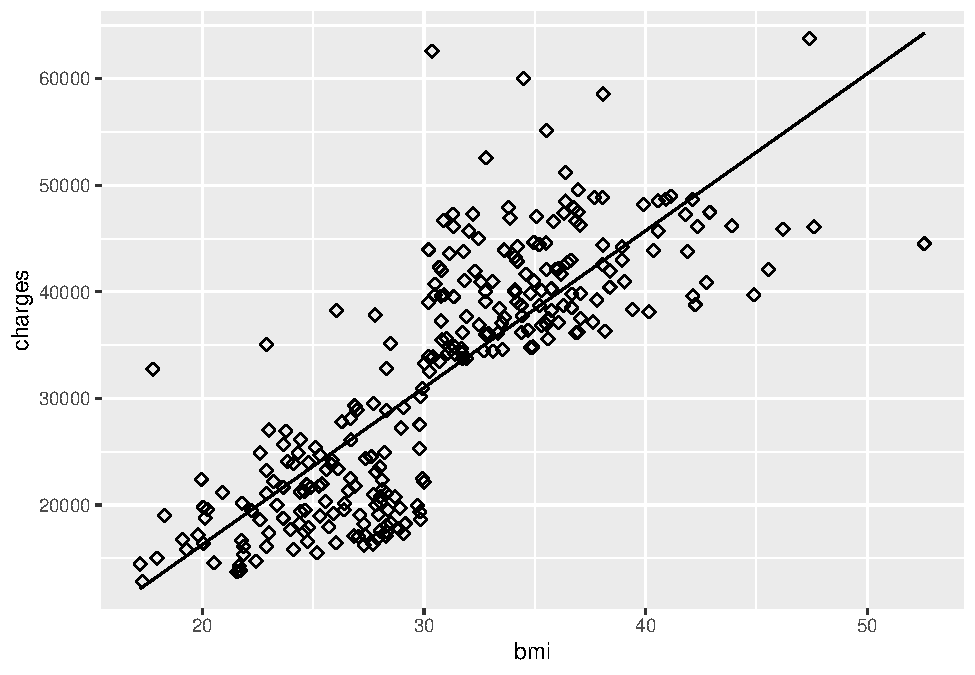
\includegraphics{Enunciado_Tarea_3_files/figure-latex/unnamed-chunk-17-1.pdf}

\begin{Shaded}
\begin{Highlighting}[]
\FunctionTok{ggplot}\NormalTok{(no\_fumadores, }\FunctionTok{aes}\NormalTok{(}\AttributeTok{x=}\NormalTok{age, }\AttributeTok{y=}\NormalTok{charges)) }\SpecialCharTok{+}
  \FunctionTok{geom\_point}\NormalTok{(}\AttributeTok{size=}\DecValTok{2}\NormalTok{, }\AttributeTok{shape=}\DecValTok{23}\NormalTok{) }\SpecialCharTok{+}
  \FunctionTok{geom\_line}\NormalTok{(}\AttributeTok{y =}\NormalTok{ (no\_fum\_age[}\DecValTok{1}\NormalTok{, }\DecValTok{1}\NormalTok{] }\SpecialCharTok{+} \FunctionTok{sort}\NormalTok{(no\_fumadores}\SpecialCharTok{$}\NormalTok{age) }\SpecialCharTok{*}\NormalTok{ no\_fum\_age[}\DecValTok{1}\NormalTok{, }\DecValTok{2}\NormalTok{]))}
\end{Highlighting}
\end{Shaded}

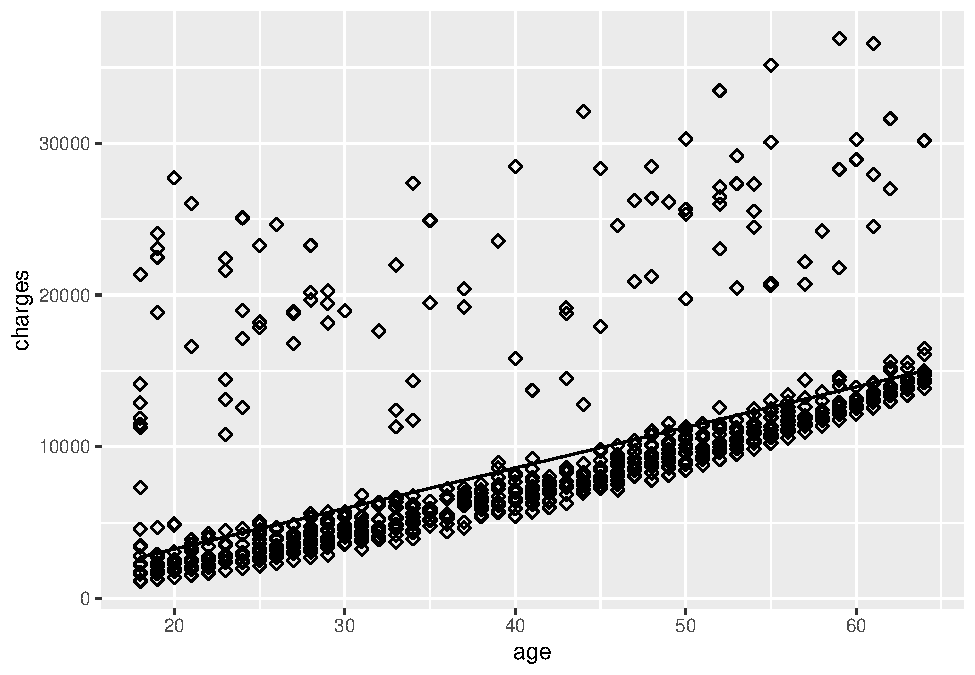
\includegraphics{Enunciado_Tarea_3_files/figure-latex/unnamed-chunk-18-1.pdf}

\hypertarget{parte-ii}{%
\paragraph{Parte II}\label{parte-ii}}

\begin{enumerate}
\def\labelenumi{\alph{enumi})}
\tightlist
\item
  Entrene un modelo lineal multivariable escogiendo dos variables
  numéricas que posean la mayor relación con \texttt{charges}.
\item
  Estudie si el modelo multivariable posee mejor desempeño que el modelo
  simple y comente los resultados. ¿Es recomendable la utilización de
  los modelos creados para la predicción de nuevas entradas?. Para este
  análisis puede utilizar los valores de test de hipótesis entregados
  por el comando \texttt{lm()}, ya que esto le servirá para observar si
  la regresión lineal es significativa.
\end{enumerate}

\textbf{Nota:} No esta permitido utilizar comandos que obtengan los
valores solicitados directamente a menos que se le permita en la
pregunta.

\begin{Shaded}
\begin{Highlighting}[]
\NormalTok{lm\_reg }\OtherTok{\textless{}{-}} \ControlFlowTok{function}\NormalTok{(X, Y)\{}
\NormalTok{  X}\SpecialCharTok{$}\NormalTok{Intercepto }\OtherTok{=} \DecValTok{1}  
  
\NormalTok{  X }\OtherTok{\textless{}{-}} \FunctionTok{as.matrix}\NormalTok{(X)}
\NormalTok{  Y }\OtherTok{\textless{}{-}} \FunctionTok{as.matrix}\NormalTok{(Y)}
  
\NormalTok{  u1 }\OtherTok{\textless{}{-}} \FunctionTok{solve}\NormalTok{(}\FunctionTok{t}\NormalTok{(X) }\SpecialCharTok{\%*\%}\NormalTok{ X)}
  
\NormalTok{  u1 }\SpecialCharTok{\%*\%} \FunctionTok{t}\NormalTok{(X) }\SpecialCharTok{\%*\%}\NormalTok{ Y}
  
\NormalTok{\}}
\end{Highlighting}
\end{Shaded}

Usando la misma correlación y resultados de la primera parte de la
pregunta: - Para fumadores se utilizarán los factores `bmi' y `age'. -
Para no fumadores se utilizarán `children' y `age'.

\begin{Shaded}
\begin{Highlighting}[]
\NormalTok{res\_fum }\OtherTok{\textless{}{-}} \FunctionTok{lm\_reg}\NormalTok{(fumadores[}\FunctionTok{c}\NormalTok{(}\DecValTok{1}\NormalTok{, }\DecValTok{2}\NormalTok{)], fumadores[}\FunctionTok{c}\NormalTok{(}\DecValTok{5}\NormalTok{)])}
\NormalTok{res\_no\_fum }\OtherTok{\textless{}{-}} \FunctionTok{lm\_reg}\NormalTok{(no\_fumadores[}\FunctionTok{c}\NormalTok{(}\DecValTok{1}\NormalTok{, }\DecValTok{3}\NormalTok{)], no\_fumadores[}\FunctionTok{c}\NormalTok{(}\DecValTok{5}\NormalTok{)])}

\NormalTok{res\_fum\_teorico\_single }\OtherTok{\textless{}{-}} \FunctionTok{lm}\NormalTok{(charges}\SpecialCharTok{\textasciitilde{}}\NormalTok{bmi, fumadores)}
\NormalTok{res\_no\_fum\_teorico\_single }\OtherTok{\textless{}{-}} \FunctionTok{lm}\NormalTok{(charges}\SpecialCharTok{\textasciitilde{}}\NormalTok{age, fumadores)}
\FunctionTok{summary}\NormalTok{(res\_fum\_teorico\_single)}\SpecialCharTok{$}\NormalTok{adj.r.squared}
\end{Highlighting}
\end{Shaded}

\begin{verbatim}
## [1] 0.6491257
\end{verbatim}

\begin{Shaded}
\begin{Highlighting}[]
\FunctionTok{summary}\NormalTok{(res\_no\_fum\_teorico\_single)}\SpecialCharTok{$}\NormalTok{adj.r.squared}
\end{Highlighting}
\end{Shaded}

\begin{verbatim}
## [1] 0.1324113
\end{verbatim}

\begin{Shaded}
\begin{Highlighting}[]
\NormalTok{res\_fum\_teorico }\OtherTok{\textless{}{-}} \FunctionTok{lm}\NormalTok{(charges}\SpecialCharTok{\textasciitilde{}}\NormalTok{age}\SpecialCharTok{+}\NormalTok{bmi, fumadores)}
\NormalTok{res\_no\_fum\_teorico }\OtherTok{\textless{}{-}} \FunctionTok{lm}\NormalTok{(charges}\SpecialCharTok{\textasciitilde{}}\NormalTok{age}\SpecialCharTok{+}\NormalTok{children, no\_fumadores)}
\FunctionTok{summary}\NormalTok{(res\_fum\_teorico)}\SpecialCharTok{$}\NormalTok{adj.r.squared}
\end{Highlighting}
\end{Shaded}

\begin{verbatim}
## [1] 0.7514192
\end{verbatim}

\begin{Shaded}
\begin{Highlighting}[]
\FunctionTok{summary}\NormalTok{(res\_no\_fum\_teorico)}\SpecialCharTok{$}\NormalTok{adj.r.squared}
\end{Highlighting}
\end{Shaded}

\begin{verbatim}
## [1] 0.4071314
\end{verbatim}

Bajo la comparación con la fumción \emph{lm()} integrada en R,
observamos que los valores son los correctos. Con respecto a si los
modelos lineales con un factor son mejores predictores o no frente a
aquellos modelos multivariable, la respuesta es que no. Los modelos
multivariables presentan un coeficiente \(R^2\,ajustado\) mayor a los de
una variable, dándonos claves importantes de que en este caso predijeron
los datos.

~

A work by CC6104

~


\end{document}
